\documentclass{beamer}

\usetheme{Madrid}
\usecolortheme{default}

\usepackage{graphicx}
\usepackage{amsmath}
\usepackage{booktabs}
\usepackage{hyperref}
\usepackage{caption}

\title[DREAMGEN]{DREAMGEN: Unlocking Generalization in Robot Learning through Video World Models}
\author[Jang et al.]{Joel Jang, Seonghyeon Ye, Zongyu Lin, Jiannan Xiang, Johan Bjorck, Yu Fang,\\
Fengyuan Hu, Spencer Huang, Kaushil Kundalia, Lin Yen-Chen, Loic Magne,\\
Ajay Mandlekar, Avnish Narayan, You Liang Tan, Guanzhi Wang, Jing Wang,\\
Qi Wang, Yinzhen Xu, Xiaohui Zeng, Kaiyuan Zheng, Ruijie Zheng, Ming-Yu Liu,\\
Luke Zettlemoyer, Dieter Fox, Jan Kautz, Scott Reed, Yuke Zhu, Linxi Fan}
\institute[NVIDIA et al.]{
NVIDIA \and University of Washington \and KAIST \and UCLA \and UCSD \and CalTech \and NTU \and University of Maryland \and UT Austin}
\date{arXiv:2505.12705v2, 2025}

\begin{document}

%------------------------------------------------
\begin{frame}
  \titlepage
\end{frame}

%------------------------------------------------
\begin{frame}
  \frametitle{Citation}
  \small
  \begin{itemize}
    \item Jang, J., Ye, S., Lin, Z., Xiang, J., Bjorck, J., Fang, Y., Hu, F., Huang, S., Kundalia, K., Yen-Chen, L., Magne, L., Mandlekar, A., Narayan, A., Tan, Y. L., Wang, G., Wang, J., Wang, Q., Xu, Y., Zeng, X., Zheng, K., Zheng, R., Liu, M.-Y., Zettlemoyer, L., Fox, D., Kautz, J., Reed, S., Zhu, Y., \& Fan, L. (2025).
    \item \textbf{DREAMGEN: Unlocking Generalization in Robot Learning through Video World Models}.
    \item arXiv preprint \texttt{arXiv:2505.12705v2 [cs.RO]}, 17 Jun 2025.
    \item URL: \url{https://research.nvidia.com/labs/gear/dreamgen}
  \end{itemize}
\end{frame}

%------------------------------------------------
\begin{frame}
  \frametitle{Research Area and Background}
  \small
  \begin{itemize}
    \item Robot foundation models trained on large-scale human teleoperation data show strong potential for general-purpose robotics \cite[Sec. 1]{}
    \item Current paradigm relies on manual teleoperation data for every new task and environment (costly, labor-intensive)
    \item Synthetic data in simulation is appealing but:
      \begin{itemize}
        \item Requires significant manual engineering
        \item Suffers from sim2real gap for visuomotor policies
      \end{itemize}
    \item Video generative models (``video world models'') have strong priors for physical reasoning, naturalistic motion, and language grounding
    \item Prior work mainly uses video world models as \emph{test-time planners}, not as large-scale data generators
  \end{itemize}
\end{frame}

%------------------------------------------------
\begin{frame}
  \frametitle{Goal of the Research}
  \small
  \begin{itemize}
    \item Propose a simple, general pipeline (\textbf{DREAMGEN}) to:
      \begin{itemize}
        \item Generate large-scale, realistic synthetic robot data from video world models
        \item Extract pseudo-actions to form \emph{neural trajectories}
        \item Train visuomotor policies that generalize across behaviors and environments
      \end{itemize}
    \item Demonstrate:
      \begin{itemize}
        \item Data augmentation benefits in simulation (RoboCasa) and real-world robots
        \item Behavior generalization to novel verbs unseen in teleoperation data
        \item Environment generalization to unseen environments from a single training environment
      \end{itemize}
    \item Introduce \textbf{DreamGen Bench} to benchmark video world models for robotics
  \end{itemize}
\end{frame}

%------------------------------------------------
\begin{frame}
  \frametitle{State of the Art and Limitations}
  \small
  \begin{itemize}
    \item Large-scale teleoperation-based robot foundation models (e.g., RT-2, GR00T N1, $\pi_0$) require extensive manual data collection
    \item Simulation-based synthetic data:
      \begin{itemize}
        \item Efficient but limited by sim2real gap and difficulty modeling liquids, deformables, articulated objects
        \item Often bounded by TAMP systems or interpolation of human demos
      \end{itemize}
    \item Generative augmentation (image/video in-painting, video2video):
      \begin{itemize}
        \item Mainly increases visual robustness
        \item Limited diversity of robot motions and behaviors
      \end{itemize}
    \item Video world models used as planners require real-time inference and tight coupling with policy, limiting scalability
  \end{itemize}
\end{frame}

%------------------------------------------------
\begin{frame}
  \frametitle{Research Motivation}
  \small
  \begin{itemize}
    \item Manual teleoperation does not scale to the diversity of tasks and environments desired for generalist robots
    \item Simulation cannot easily capture complex real-world physics (tools, deformables, liquids)
    \item Video world models already encode:
      \begin{itemize}
        \item Internet-scale knowledge of physics and everyday scenes
        \item Language grounding and visual dynamics
      \end{itemize}
    \item Treating video world models as \emph{offline synthetic data generators} could:
      \begin{itemize}
        \item Decouple heavy video generation from policy execution
        \item Enable large-scale, low-labor data generation for many robots and tasks
      \end{itemize}
  \end{itemize}
\end{frame}

%------------------------------------------------
\begin{frame}
  \frametitle{Problem Definition}
  \small
  \begin{itemize}
    \item Input:
      \begin{itemize}
        \item Limited human teleoperation trajectories for a given robot embodiment (often only pick-and-place in one environment)
        \item A pretrained video world model
      \end{itemize}
    \item Desired output:
      \begin{itemize}
        \item Visuomotor policies that:
          \begin{itemize}
            \item Perform well on existing tasks
            \item Generalize to novel behaviors (new verbs)
            \item Generalize to novel environments (new scenes)
          \end{itemize}
      \end{itemize}
    \item Constraints:
      \begin{itemize}
        \item Minimize additional teleoperation data
        \item Use only video world models that output videos (no direct actions)
        \item Maintain physical plausibility and instruction following in generated data
      \end{itemize}
  \end{itemize}
\end{frame}

%------------------------------------------------
\begin{frame}
  \frametitle{Proposed Method: DREAMGEN Pipeline}
  \small
  \begin{itemize}
    \item 4-stage pipeline (Fig. 2, p.2):
      \begin{enumerate}
        \item \textbf{Fine-tune} video world model on teleoperated robot trajectories
        \item \textbf{Roll out} video world model with initial frames + language instructions
        \item \textbf{Label pseudo-actions} via IDM or latent action model (LAPA)
        \item \textbf{Train visuomotor policies} on resulting neural trajectories
      \end{enumerate}
    \item Neural trajectories: video-action sequence pairs generated entirely by the world model + pseudo-action extractor
    \item Applicable across robots (GR1 humanoid, Franka, SO-100), tasks, and environments
  \end{itemize}
\end{frame}

%------------------------------------------------
\begin{frame}
  \frametitle{Method: Video World Model Fine-tuning}
  \small
  \begin{itemize}
    \item Base models: state-of-the-art video generative models (e.g., WAN 2.1) \cite[Sec. 2.1]{}
    \item Fine-tuning:
      \begin{itemize}
        \item Use LoRA to adapt to target robot while mitigating forgetting of internet video knowledge
        \item Train on human teleoperation trajectories per embodiment (RoboCasa, GR1, DROID, SO-100)
      \end{itemize}
    \item Evaluation criteria during fine-tuning:
      \begin{itemize}
        \item Instruction following
        \item Physics following
      \end{itemize}
    \item Multiview data (RoboCasa, DROID):
      \begin{itemize}
        \item Concatenate views into 2$\times$2 grid (one black cell) for training
      \end{itemize}
  \end{itemize}
\end{frame}

%------------------------------------------------
\begin{frame}
  \frametitle{Method: Video World Model Rollout}
  \small
  \begin{itemize}
    \item After fine-tuning, generate synthetic robot videos:
      \begin{itemize}
        \item Condition on initial frame $o_1$
        \item Condition on language instruction $i$ (e.g., ``water the flowers'')
      \end{itemize}
    \item Initial frames:
      \begin{itemize}
        \item Simulation: sampled from simulator with randomized object locations/environments
        \item Real world: manually captured with randomized target object positions
        \item Environment generalization: initial frames from 10 new environments, while training data from a single environment
      \end{itemize}
    \item Behavior generalization:
      \begin{itemize}
        \item Manually design novel behavior prompts (new verbs)
        \item Include prompts from DreamGen Bench
      \end{itemize}
  \end{itemize}
\end{frame}

%------------------------------------------------
\begin{frame}
  \frametitle{Method: Pseudo-Action Labeling}
  \small
  \begin{itemize}
    \item Two mechanisms (Fig. 3, p.4):
      \begin{itemize}
        \item \textbf{Inverse Dynamics Model (IDM)} actions
        \item \textbf{Latent actions} via LAPA
      \end{itemize}
    \item IDM:
      \begin{itemize}
        \item Diffusion transformer with SigLIP-2 vision encoder
        \item Conditioned on two frames, predicts action chunks between them
        \item Trained with flow-matching objective on same data as video world model
        \item Sliding window over generated videos to obtain dense pseudo-actions
      \end{itemize}
    \item LAPA:
      \begin{itemize}
        \item Transformer encoder-decoder with VQ-VAE objective
        \item Trained on diverse robot and human videos (Table 3, p.15)
        \item Condition on current frame and future frame (1s ahead)
        \item Use pre-quantized continuous embedding as latent action
      \end{itemize}
  \end{itemize}
\end{frame}

%------------------------------------------------
\begin{frame}
  \frametitle{Method: Policy Training on Neural Trajectories}
  \small
  \begin{itemize}
    \item Policies condition on:
      \begin{itemize}
        \item Image observation $o_t$
        \item Language instruction $i_t$
      \end{itemize}
    \item Predict action sequence $\hat{a}_{t:t+H}$:
      \begin{itemize}
        \item Either IDM actions or latent actions
      \end{itemize}
    \item State information in neural trajectories is set to zero (no state in generated videos)
    \item Policy backbones:
      \begin{itemize}
        \item Diffusion Policy
        \item $\pi_0$
        \item GR00T N1
      \end{itemize}
    \item Training regimes:
      \begin{itemize}
        \item Co-training real + neural trajectories (1:1 sampling)
        \item Training solely on neural trajectories (IDM actions)
      \end{itemize}
  \end{itemize}
\end{frame}

%------------------------------------------------
% FIGURE 1
\begin{frame}
  \frametitle{Overview Illustration (Figure 1)}
  \begin{columns}
    \begin{column}{0.5\textwidth}
      \small
      \begin{itemize}
        \item Figure 1 (p.1) illustrates DREAMGEN enabling 2D visuomotor policies to generalize to:
          \begin{itemize}
            \item New behaviors
            \item New environments
          \end{itemize}
        \item Only teleoperation data: single pick-and-place behavior in a single environment
        \item Video world model generates synthetic, photorealistic videos for diverse tasks and scenes
        \item Pseudo-actions are automatically extracted to form neural trajectories
        \item Demonstrates contact-rich data augmentation and generalization capabilities
      \end{itemize}
    \end{column}
    \begin{column}{0.5\textwidth}
      \centering
      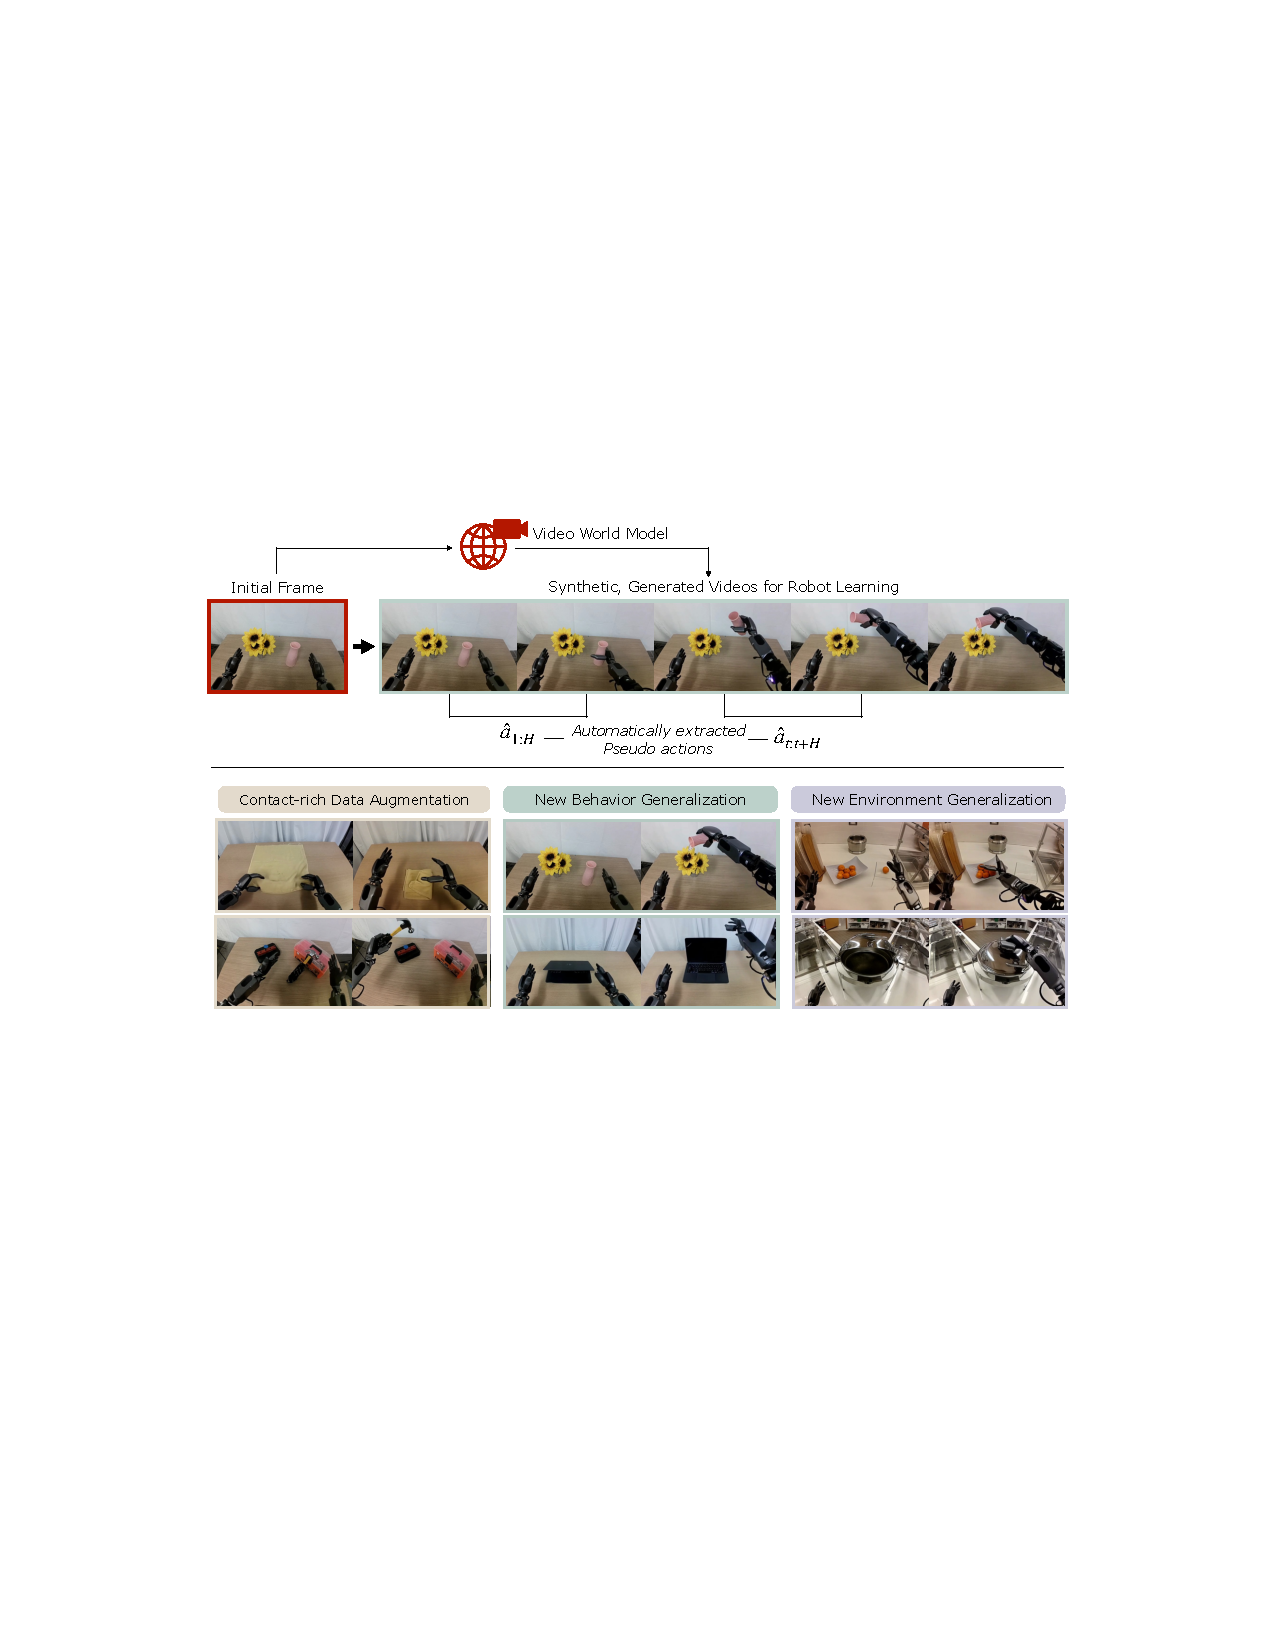
\includegraphics[width=0.7\textwidth,keepaspectratio]{extracted/figure_01.pdf}
      \captionof{figure}{Figure 1 (p.1) shows how DREAMGEN uses video world models to generate synthetic videos and unlock behavior and environment generalization from a single teleoperated behavior.}
    \end{column}
  \end{columns}
\end{frame}

%------------------------------------------------
% FIGURE 2
\begin{frame}
  \frametitle{DREAMGEN Pipeline (Figure 2)}
  \begin{columns}
    \begin{column}{0.5\textwidth}
      \small
      \begin{itemize}
        \item Figure 2 (p.2) visualizes the 4-step DREAMGEN pipeline:
          \begin{itemize}
            \item Step 1: Fine-tune video world model on teleoperated trajectories
            \item Step 2: Roll out model with initial frame + language instruction
            \item Step 3: Label pseudo-actions via IDM or LAPA
            \item Step 4: Train visuomotor policies on neural trajectories
          \end{itemize}
        \item Generated videos depict intended behaviors but lack actions; pseudo-actions fill this gap
        \item Neural trajectories are the core training data for downstream policies
      \end{itemize}
    \end{column}
    \begin{column}{0.5\textwidth}
      \centering

      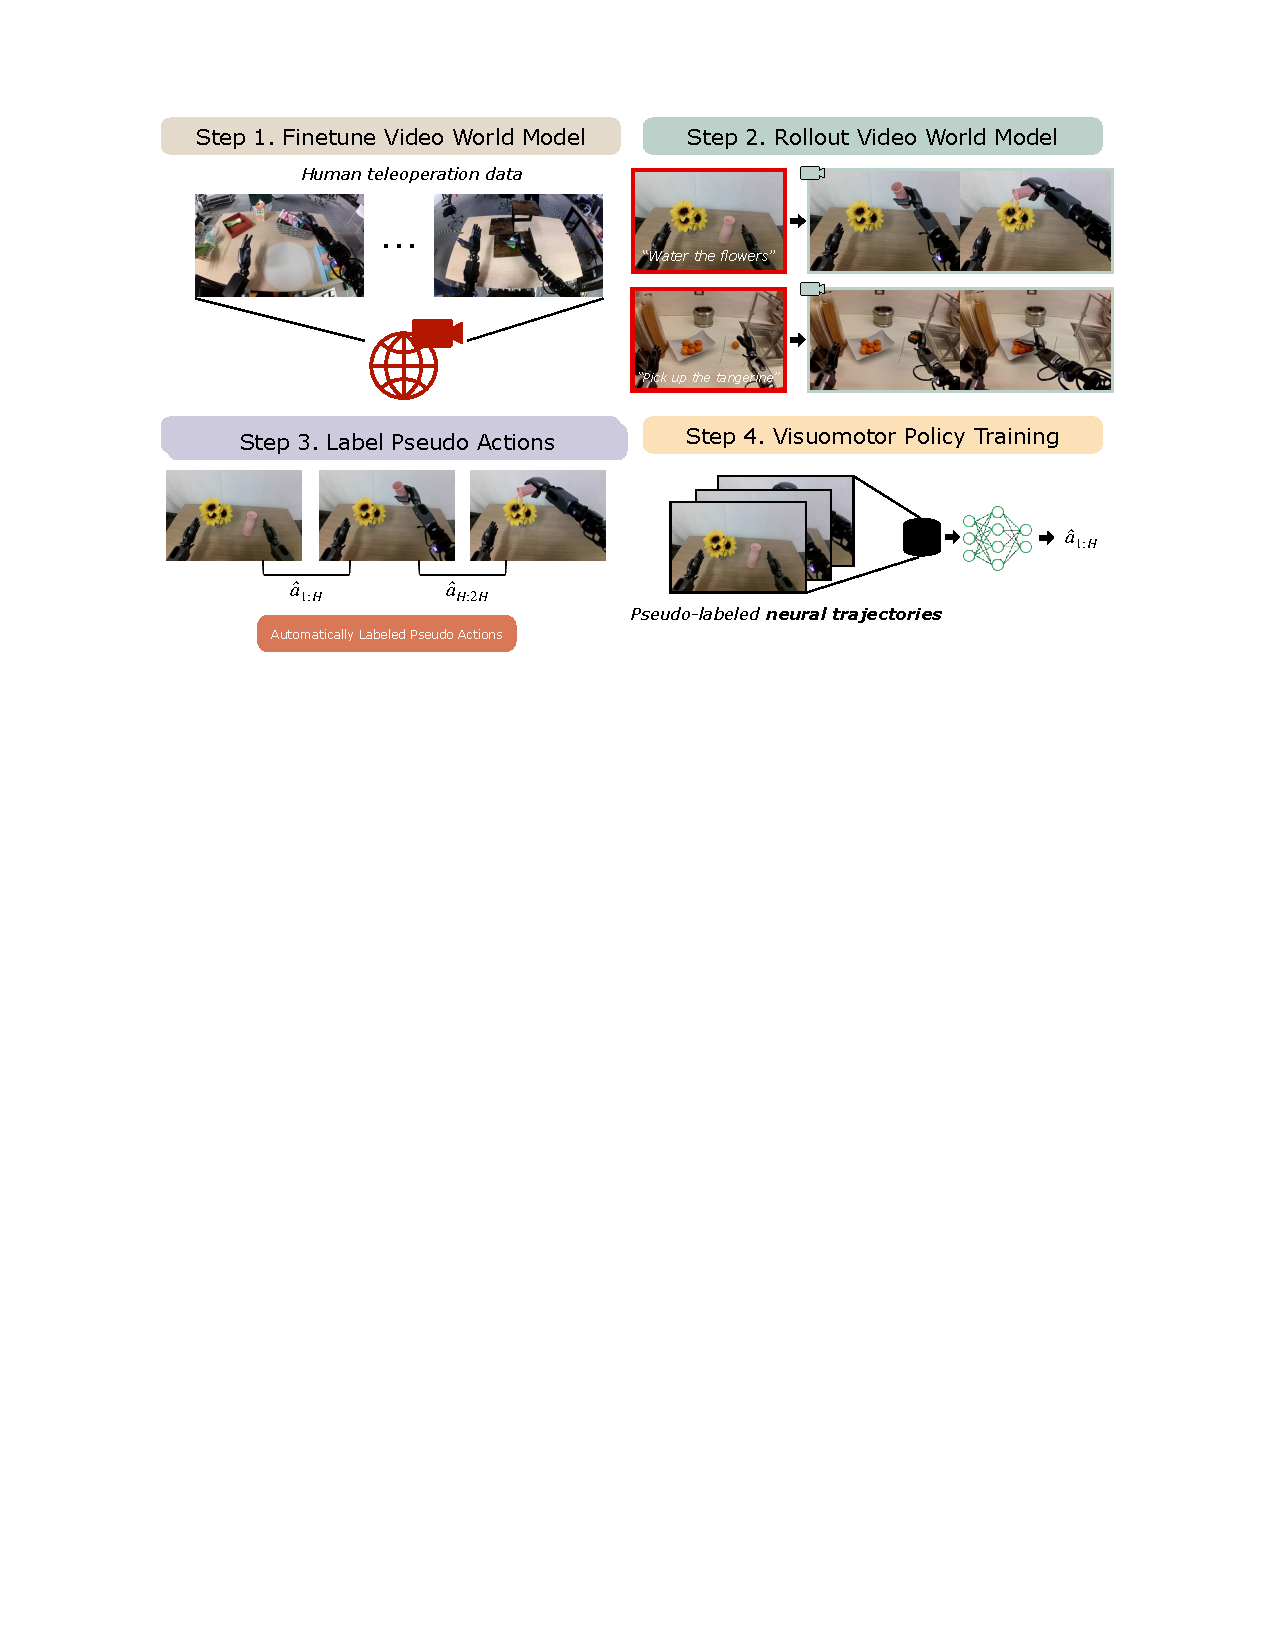
\includegraphics[width=0.7\textwidth,keepaspectratio]{extracted/figure_02.pdf}

      \captionof{figure}{Figure 2 (p.2) provides an overview of DREAMGEN: fine-tuning, rollout, pseudo-action labeling, and policy training on neural trajectories.}
    \end{column}
  \end{columns}
\end{frame}

%------------------------------------------------
% FIGURE 3
\begin{frame}
  \frametitle{Pseudo-Action Models (Figure 3)}
  \begin{columns}
    \begin{column}{0.5\textwidth}
      \small
      \begin{itemize}
        \item Figure 3 (p.4) shows architectures for:
          \begin{itemize}
            \item (a) Inverse Dynamics Model (IDM)
            \item (b) Latent action model (LAPA)
          \end{itemize}
        \item IDM:
          \begin{itemize}
            \item Vision encoder + diffusion transformer
            \item Predicts action chunks between two frames
            \item Trained with action flow-matching objective
          \end{itemize}
        \item LAPA:
          \begin{itemize}
            \item ViT encoder-decoder with VQ codebook
            \item Encodes visual deltas into discrete latent actions
          \end{itemize}
        \item Both are used to extract pseudo-actions from generated videos
      \end{itemize}
    \end{column}
    \begin{column}{0.5\textwidth}
      \centering

      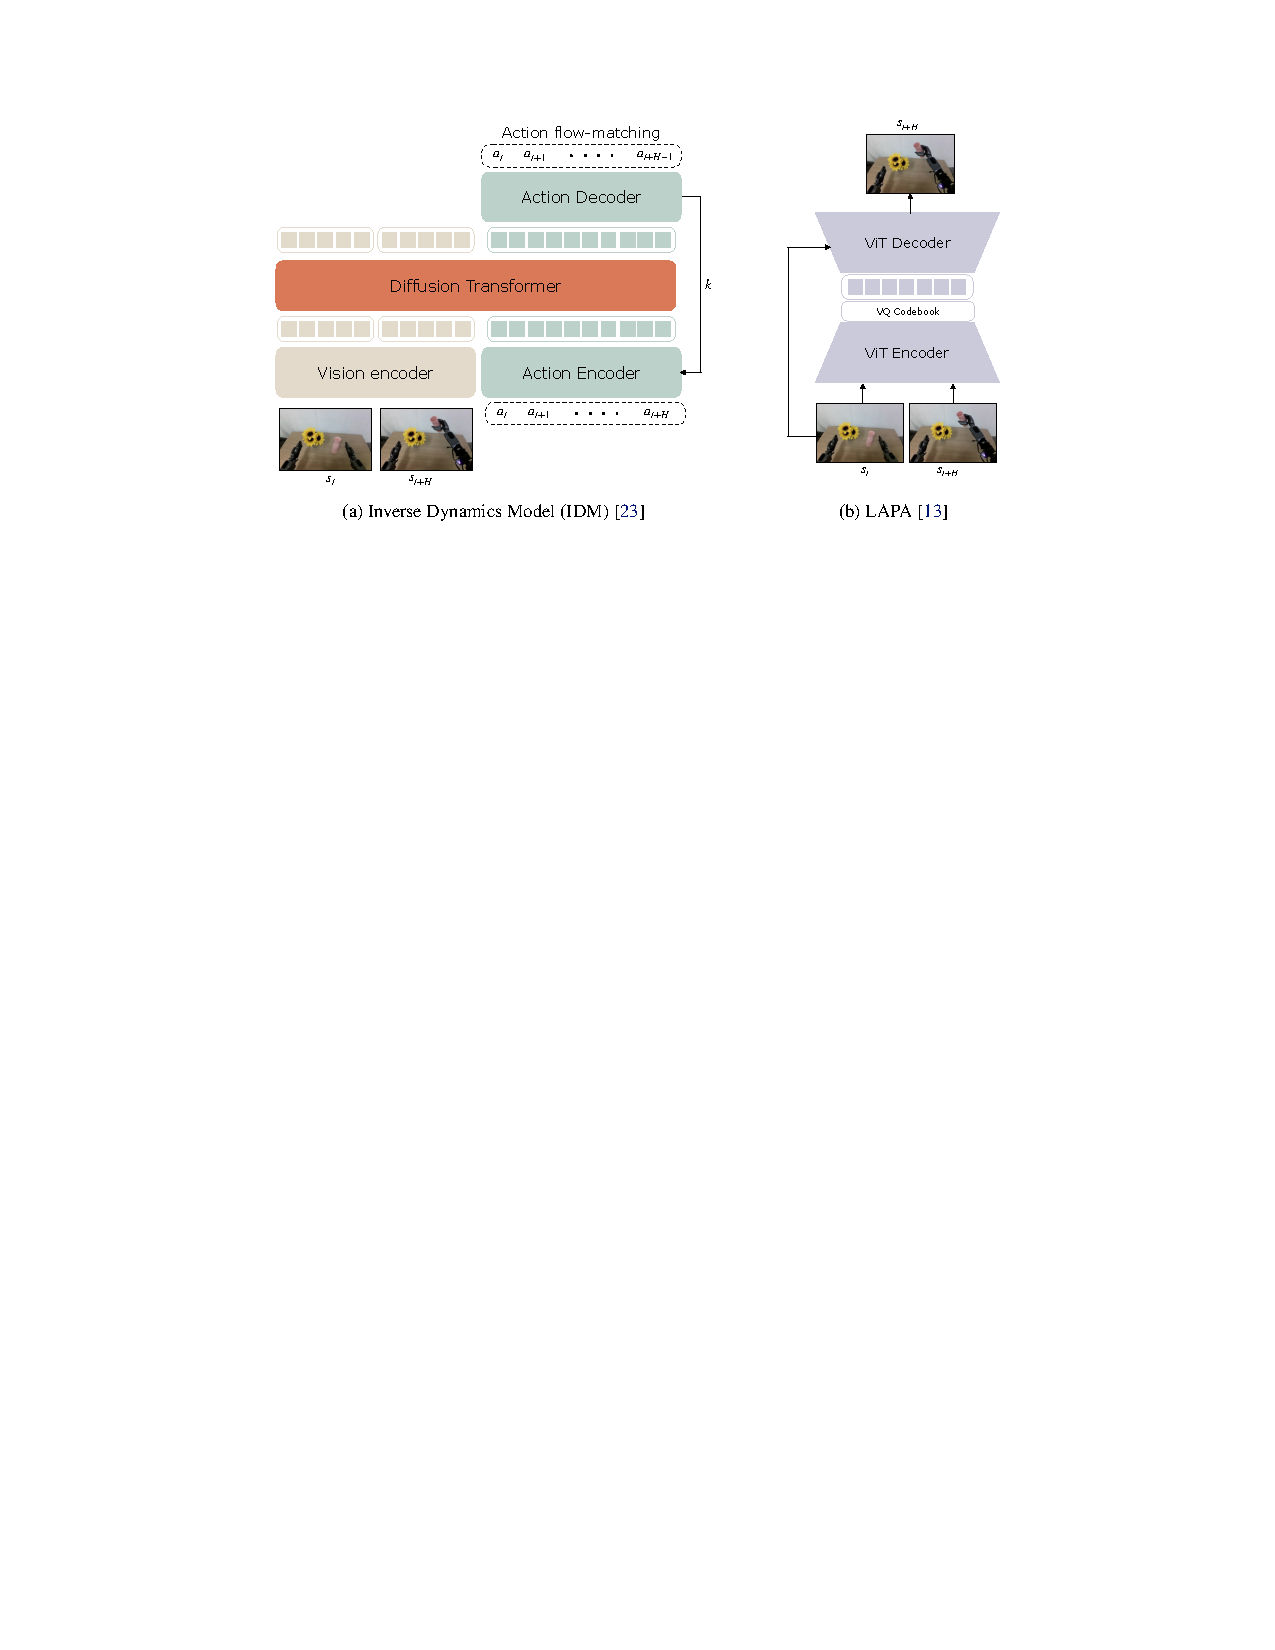
\includegraphics[width=0.7\textwidth,keepaspectratio]{extracted/figure_03.pdf}

      \captionof{figure}{Figure 3 (p.4) depicts the IDM and LAPA architectures used to extract pseudo-actions from synthetic videos.}
    \end{column}
  \end{columns}
\end{frame}

%------------------------------------------------
\begin{frame}
  \frametitle{Experimental Design}
  \small
  \begin{itemize}
    \item Three main applications (Sec. 3):
      \begin{itemize}
        \item Training data augmentation
        \item Behavior generalization
        \item Environment generalization
      \end{itemize}
    \item Simulation:
      \begin{itemize}
        \item RoboCasa benchmark (24 tasks, Franka in kitchen-like scenes)
        \item Vary ground-truth data regimes: low (720), mid (2.4k), high (7.2k)
        \item Scale neural trajectories up to 333$\times$ original demos
      \end{itemize}
    \item Real-world:
      \begin{itemize}
        \item GR1 humanoid: 4 dexterous tasks
        \item Franka: 3 manipulation tasks
        \item SO-100: 2 tasks with GR00T N1 VLA
      \end{itemize}
  \end{itemize}
\end{frame}

%------------------------------------------------
% FIGURE 4
\begin{frame}
  \frametitle{Scaling Neural Trajectories in RoboCasa (Figure 4)}
  \begin{columns}
    \begin{column}{0.5\textwidth}
      \small
      \begin{itemize}
        \item Figure 4 (p.5) plots average success rate vs.\ number of neural trajectories
        \item Three ground-truth regimes: low, mid, high; two pseudo-action types: LAPA and IDM
        \item Co-training with neural trajectories improves performance across all regimes
        \item Performance increases approximately log-linearly with number of neural trajectories
        \item Policies trained solely on IDM-based neural trajectories achieve 20.6\% average success across 24 tasks
      \end{itemize}
    \end{column}
    \begin{column}{0.5\textwidth}
      \centering

      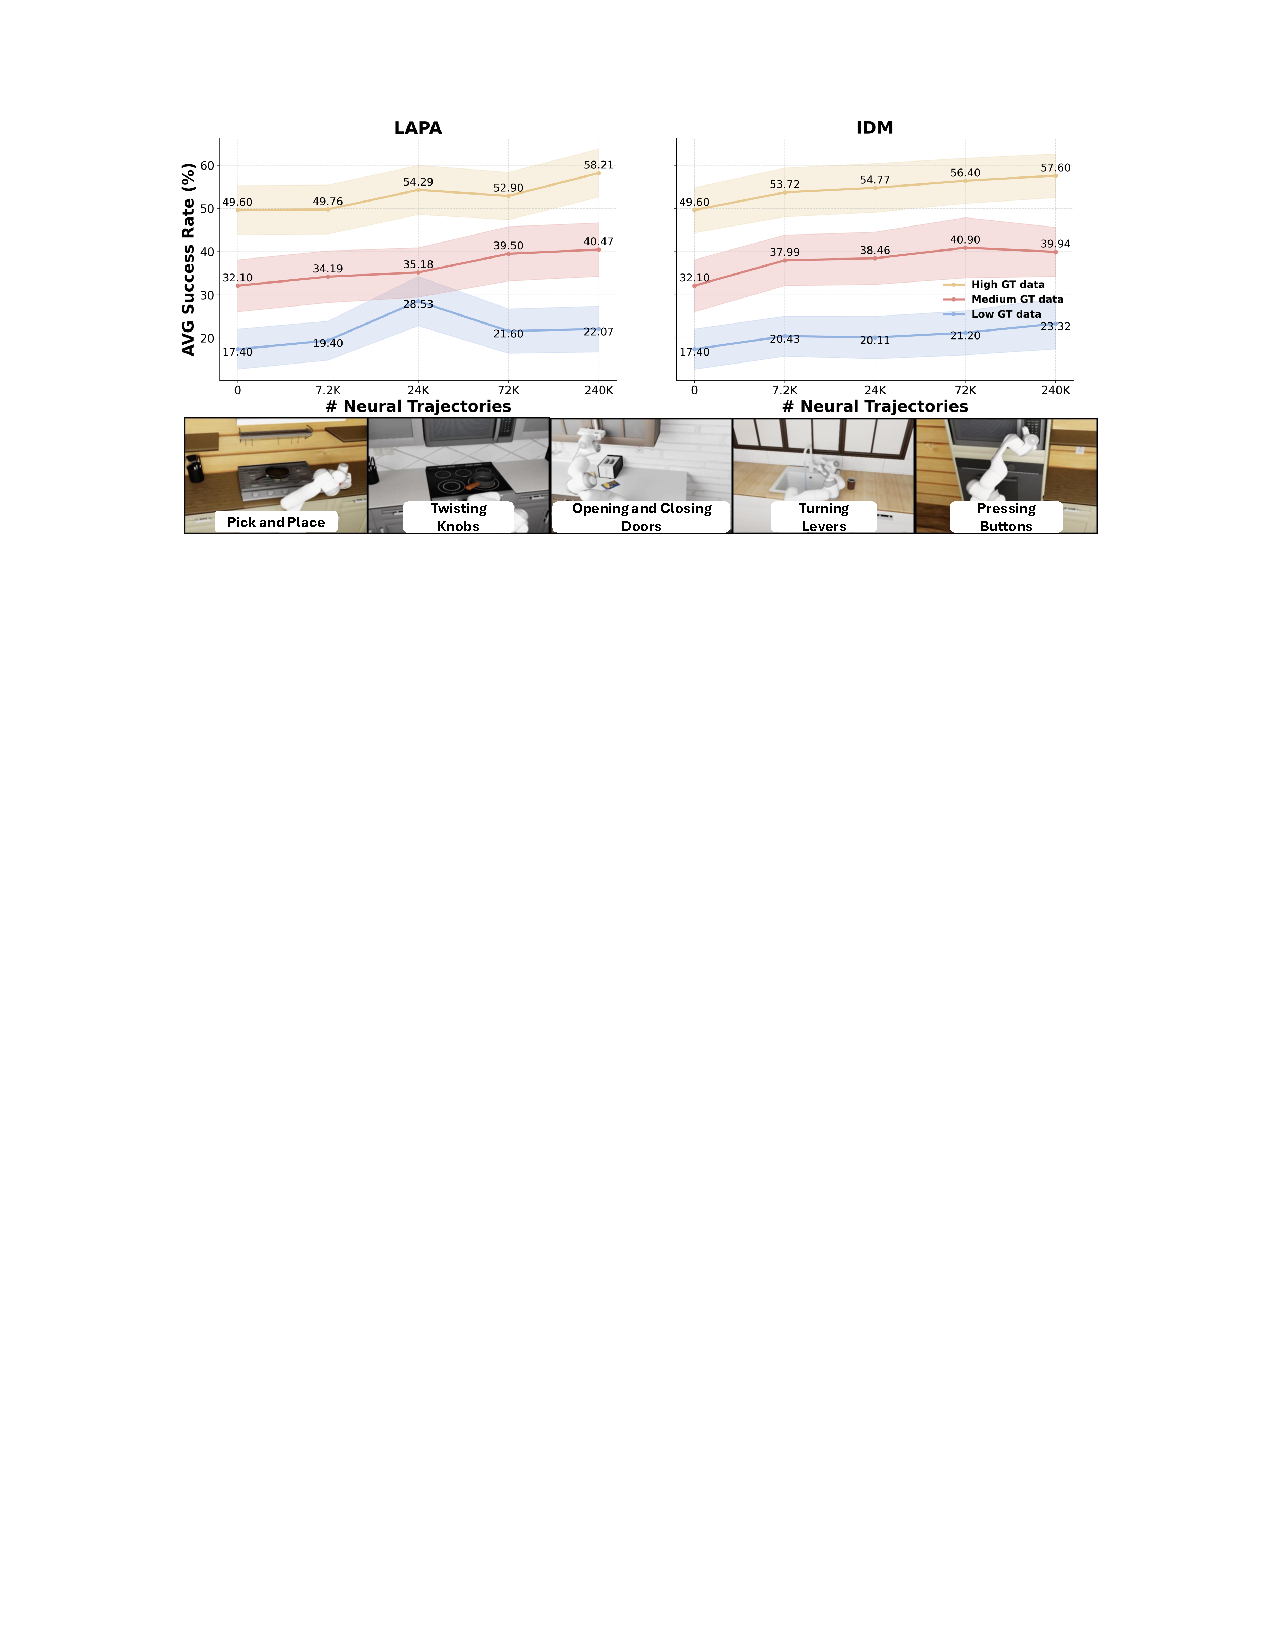
\includegraphics[width=0.7\textwidth,keepaspectratio]{extracted/figure_04.pdf}

      \captionof{figure}{Figure 4 (p.5) shows RoboCasa success rates as the number of neural trajectories increases under different ground-truth data regimes and pseudo-action types.}
    \end{column}
  \end{columns}
\end{frame}

%------------------------------------------------
% FIGURE 5
\begin{frame}
  \frametitle{Real-World Robot Evaluation (Figure 5)}
  \begin{columns}
    \begin{column}{0.5\textwidth}
      \small
      \begin{itemize}
        \item Figure 5 (p.6) summarizes real-world results on:
          \begin{itemize}
            \item GR1 humanoid (4 tasks)
            \item Franka (3 tasks)
            \item SO-100 (2 tasks)
          \end{itemize}
        \item ``Low Data'': 10\% of available trajectories (10 per task, 25 for GR1 folding; 25\% for SO-100)
        \item ``Low Data + Neural Traj.'': co-training with neural trajectories (1:1 sampling)
        \item Neural trajectories consistently improve success rates across embodiments and policies
        \item Gains are especially notable for GR00T N1, likely due to separate action encoder/decoder for IDM actions
      \end{itemize}
    \end{column}
    \begin{column}{0.5\textwidth}
      \centering

      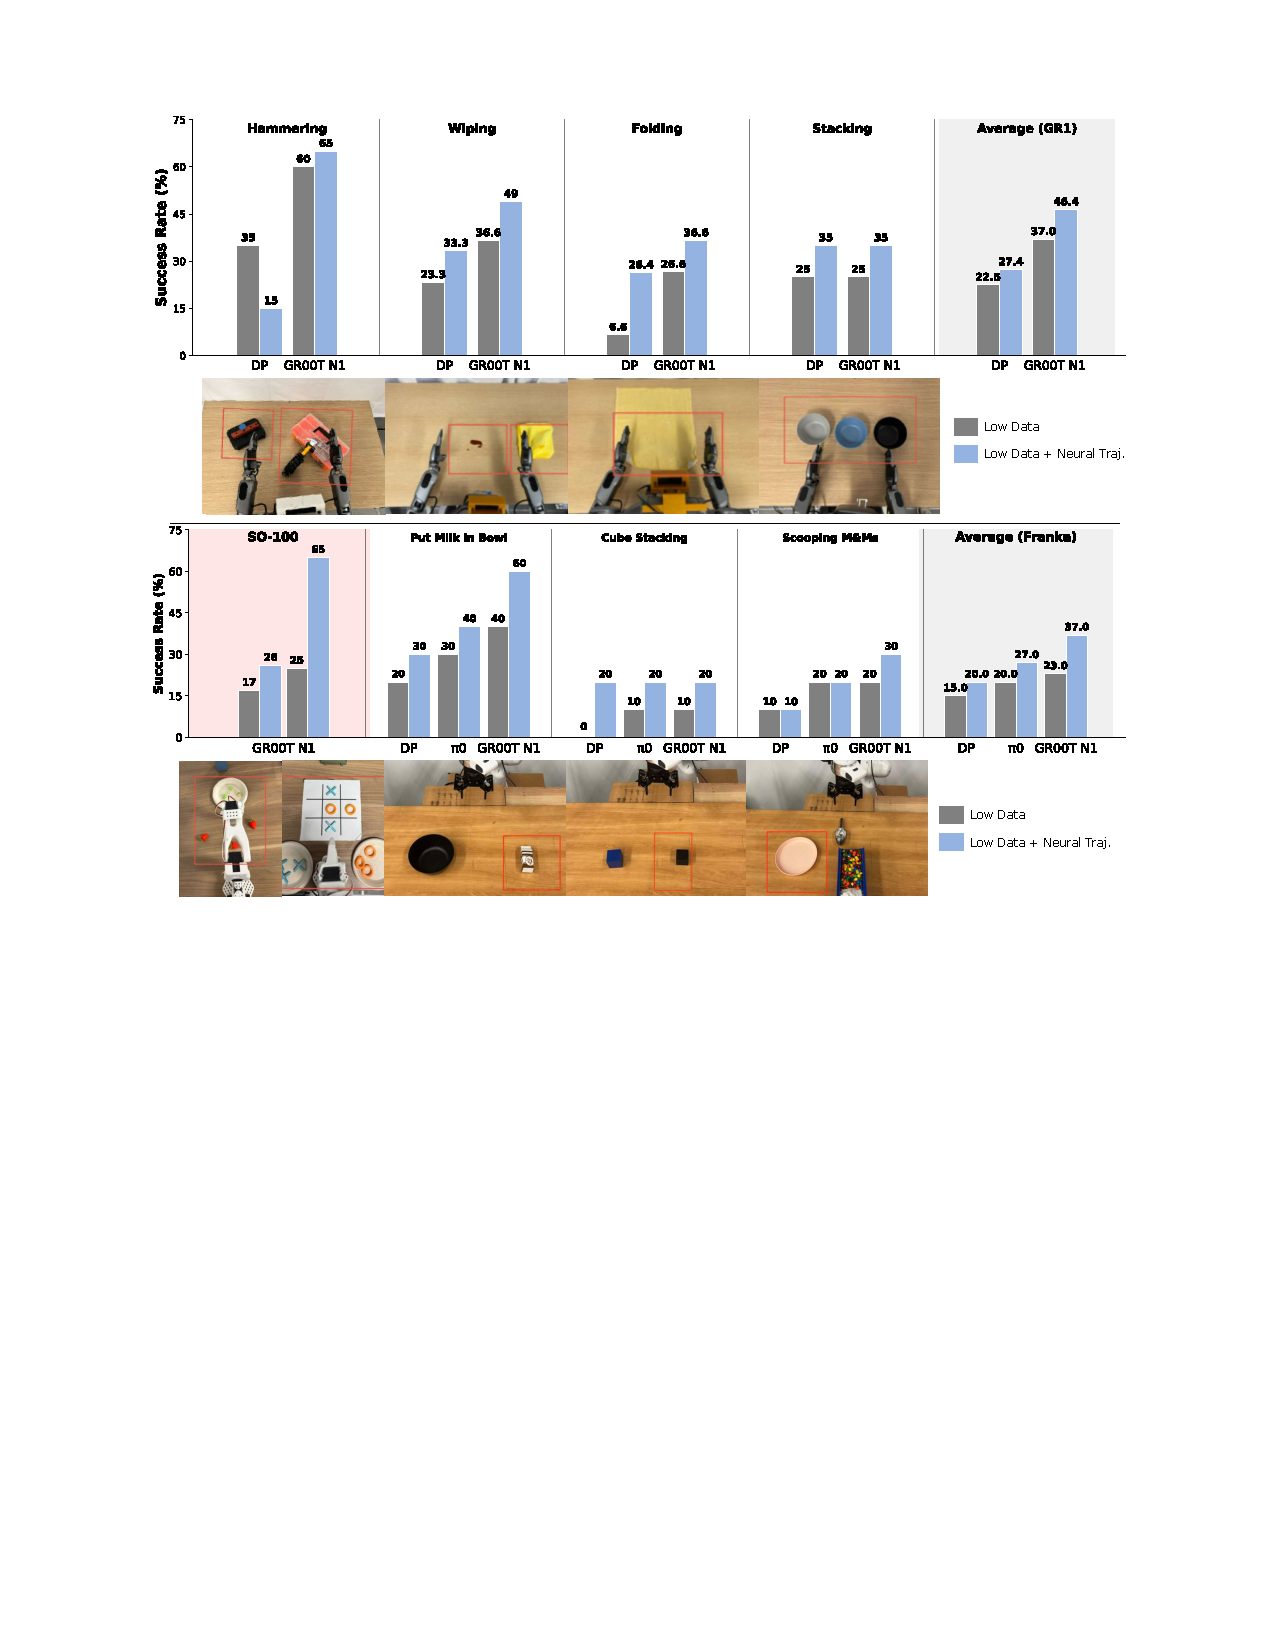
\includegraphics[width=0.7\textwidth,keepaspectratio]{extracted/figure_05.pdf}

      \captionof{figure}{Figure 5 (p.6) shows success rates for real-world GR1, Franka, and SO-100 tasks with and without co-training on neural trajectories.}
    \end{column}
  \end{columns}
\end{frame}

%------------------------------------------------
% TABLE 1
\begin{frame}
  \frametitle{Behavior and Environment Generalization (Table 1)}
  \begin{columns}
    \begin{column}{0.45\textwidth}
      \small
      \begin{itemize}
        \item Table 1 (p.7) reports success rates for:
          \begin{itemize}
            \item 14 novel behaviors in seen environments
            \item 13 tasks in novel environments (seen and novel behaviors)
          \end{itemize}
        \item Baseline GR00T N1 trained only on 2{,}884 pick-and-place trajectories:
          \begin{itemize}
            \item 11.2\% average on novel behaviors in seen envs
            \item 0\% on all tasks in novel environments
          \end{itemize}
        \item With DREAMGEN neural trajectories:
          \begin{itemize}
            \item 43.2\% average on 14 novel behaviors in seen envs
            \item 28.5\% average on 13 tasks in novel environments
          \end{itemize}
        \item Demonstrates learning entirely new verbs and zero-shot environment transfer from a single training environment
      \end{itemize}
    \end{column}
    \begin{column}{0.55\textwidth}
      \centering

      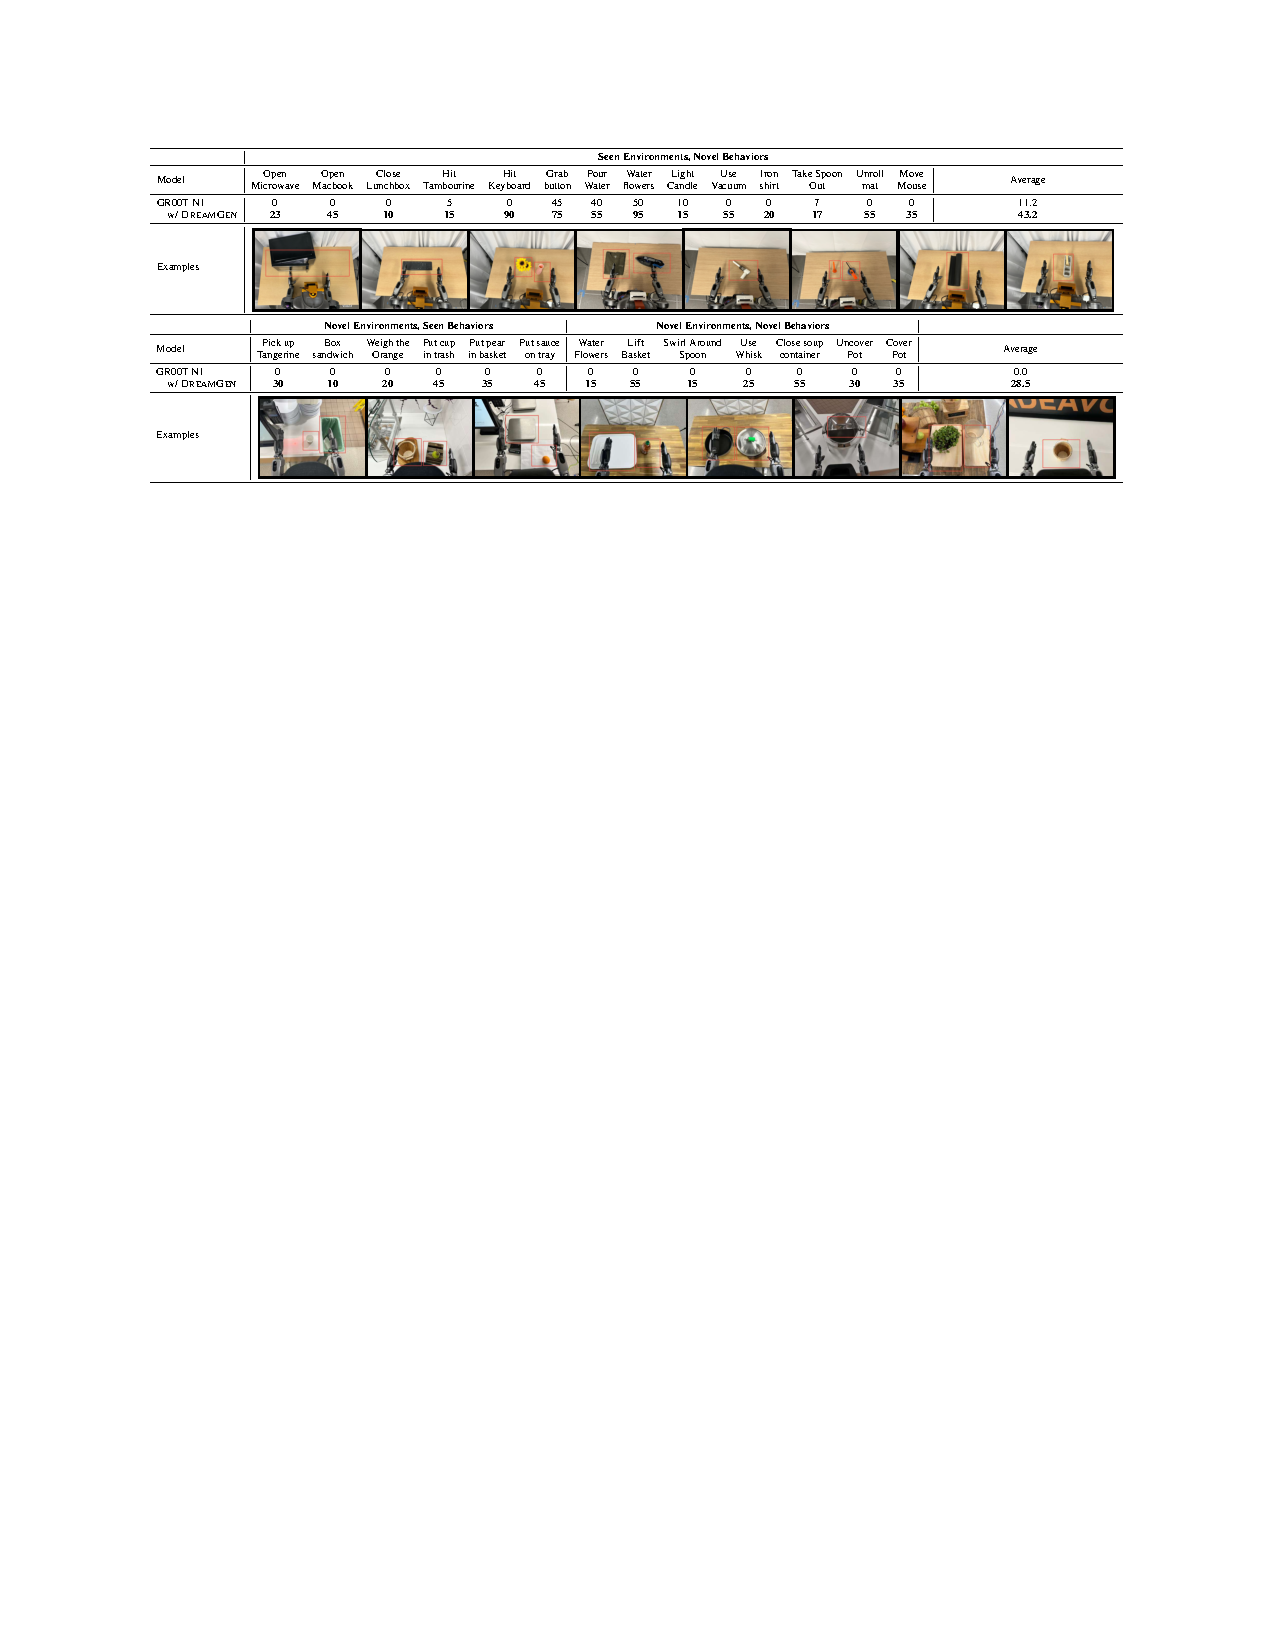
\includegraphics[width=0.9\columnwidth,keepaspectratio]{extracted/table_01.pdf}

      \captionof{figure}{Table 1 (p.7) lists success rates for GR1 on novel behaviors in seen environments and on seen/novel behaviors in novel environments, comparing GR00T N1 with and without DREAMGEN.}
    \end{column}
  \end{columns}
\end{frame}

%------------------------------------------------
\begin{frame}
  \frametitle{DreamGen Bench: Benchmark Design}
  \small
  \begin{itemize}
    \item Goal: quantify how well video world models adapt to robot embodiments and generalize to:
      \begin{itemize}
        \item Unseen objects
        \item Unseen behaviors
        \item Unseen environments
      \end{itemize}
    \item Two key metrics:
      \begin{itemize}
        \item \textbf{Instruction Following (IF)}: binary score (0/1) from VLMs (GPT-4o, Qwen2.5-VL) on whether video matches task instruction
        \item \textbf{Physics Alignment (PA)}: physical plausibility via VideoCon-Physics and Qwen2.5-VL
      \end{itemize}
    \item Datasets:
      \begin{itemize}
        \item RoboCasa (simulation, Franka)
        \item GR1 (real humanoid)
      \end{itemize}
    \item Models evaluated: Hunyuan, CogVideoX, WAN 2.1, Cosmos; zero-shot and fine-tuned variants
  \end{itemize}
\end{frame}

%------------------------------------------------
% TABLE 2
\begin{frame}
  \frametitle{DreamGen Bench Results (Table 2)}
  \begin{columns}
    \begin{column}{0.45\textwidth}
      \small
      \begin{itemize}
        \item Table 2 (p.8) summarizes:
          \begin{itemize}
            \item Dataset statistics (train trajectories, eval frames)
            \item IF and PA scores for each model and dataset
          \end{itemize}
        \item Zero-shot models generally have very low IF and PA (often near 0)
        \item Fine-tuned models substantially improve both metrics
        \item Cosmos-sft and WAN2.1-sft achieve highest IF and PA across datasets
        \item Human evaluations show $>$90\% Pearson correlation with automatic IF metrics, validating benchmark reliability
      \end{itemize}
    \end{column}
    \begin{column}{0.55\textwidth}
      \centering

      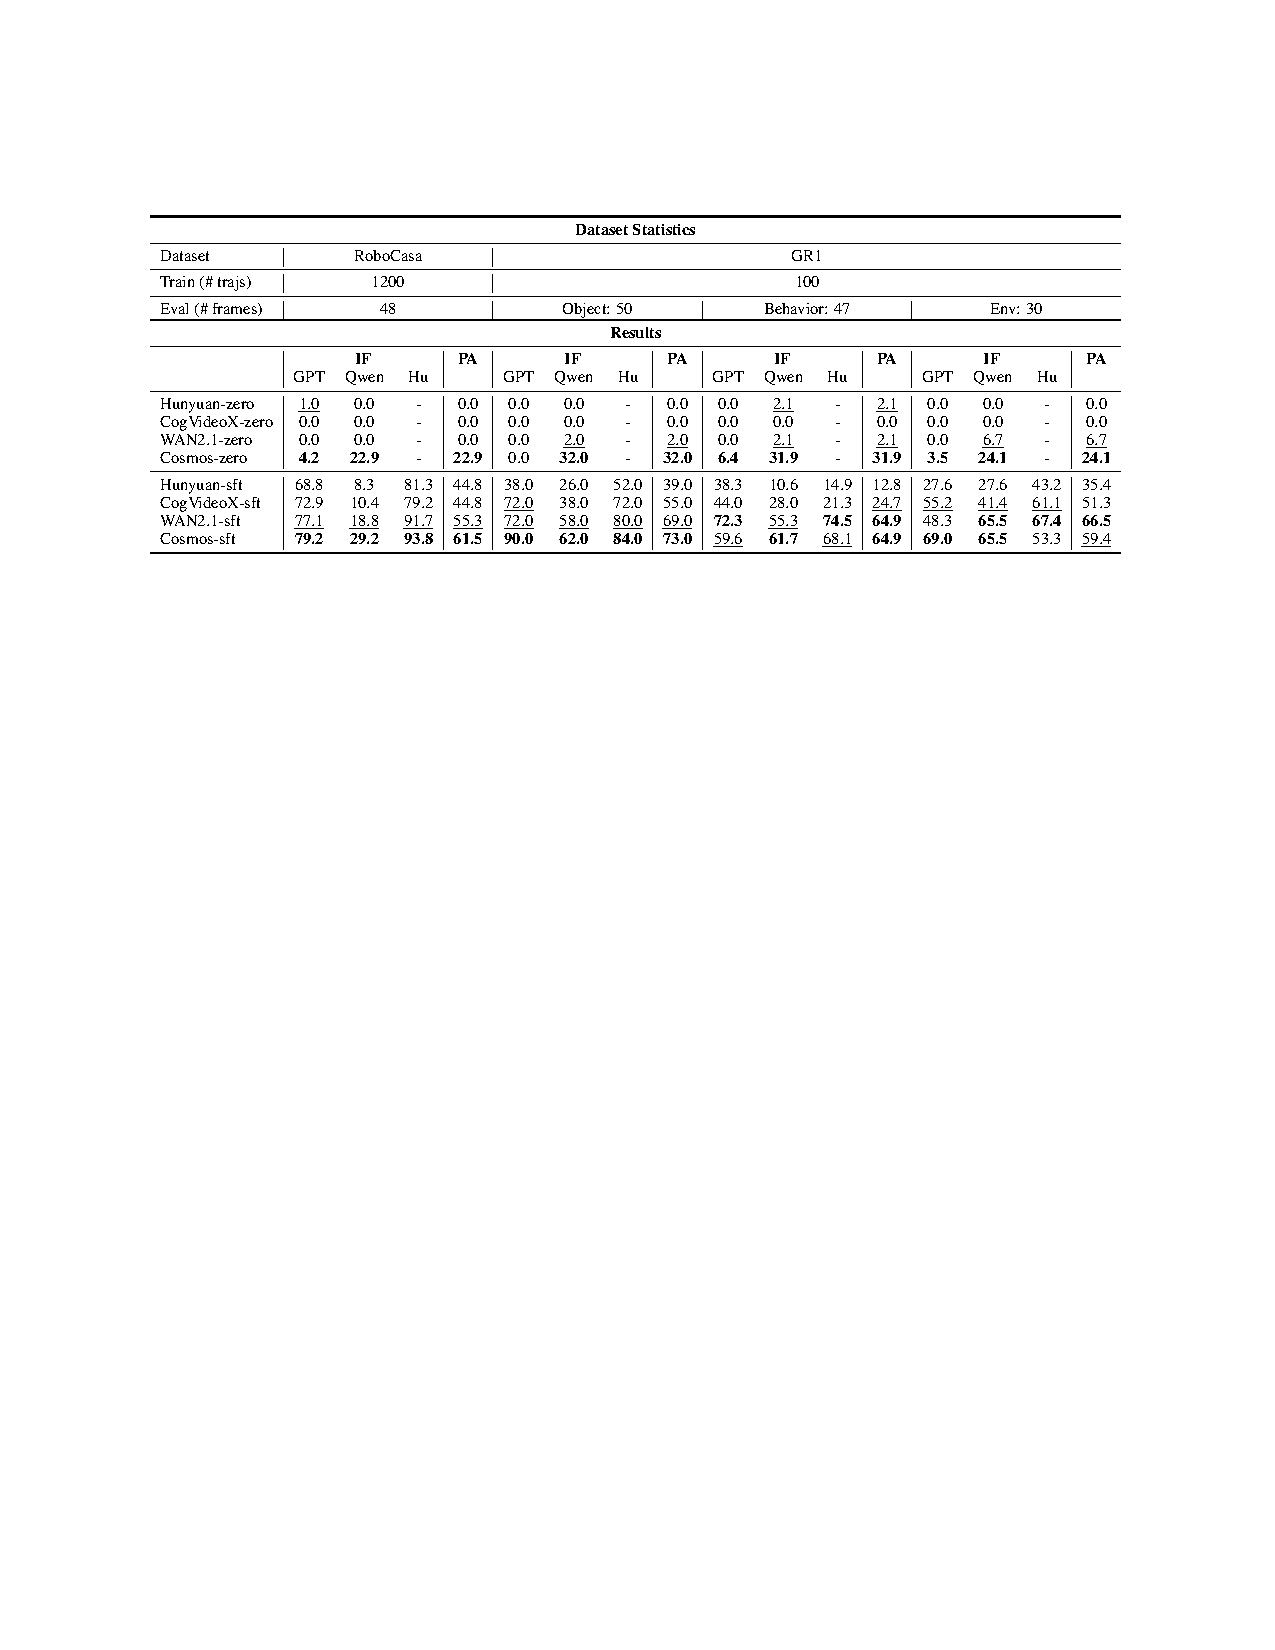
\includegraphics[width=0.9\columnwidth,keepaspectratio]{extracted/table_02.pdf}

      \captionof{figure}{Table 2 (p.8) reports DreamGen Bench statistics and IF/PA scores for multiple video world models in zero-shot and fine-tuned settings on RoboCasa and GR1.}
    \end{column}
  \end{columns}
\end{frame}

%------------------------------------------------
% FIGURE 6
\begin{frame}
  \frametitle{Correlation with Downstream Performance (Figure 6)}
  \begin{columns}
    \begin{column}{0.5\textwidth}
      \small
      \begin{itemize}
        \item Figure 6 (p.8) plots DreamGen Bench score vs.\ RoboCasa policy performance
        \item DreamGen Bench score: average of IF (GPT) and PA from Table 2
        \item RoboCasa score: success rate when training policies only on neural trajectories from each video model (7k trajectories)
        \item Positive correlation: models with higher IF/PA yield better downstream manipulation performance
        \item Indicates that improving video world models along these axes directly benefits robot learning via DREAMGEN
      \end{itemize}
    \end{column}
    \begin{column}{0.5\textwidth}
      \centering

      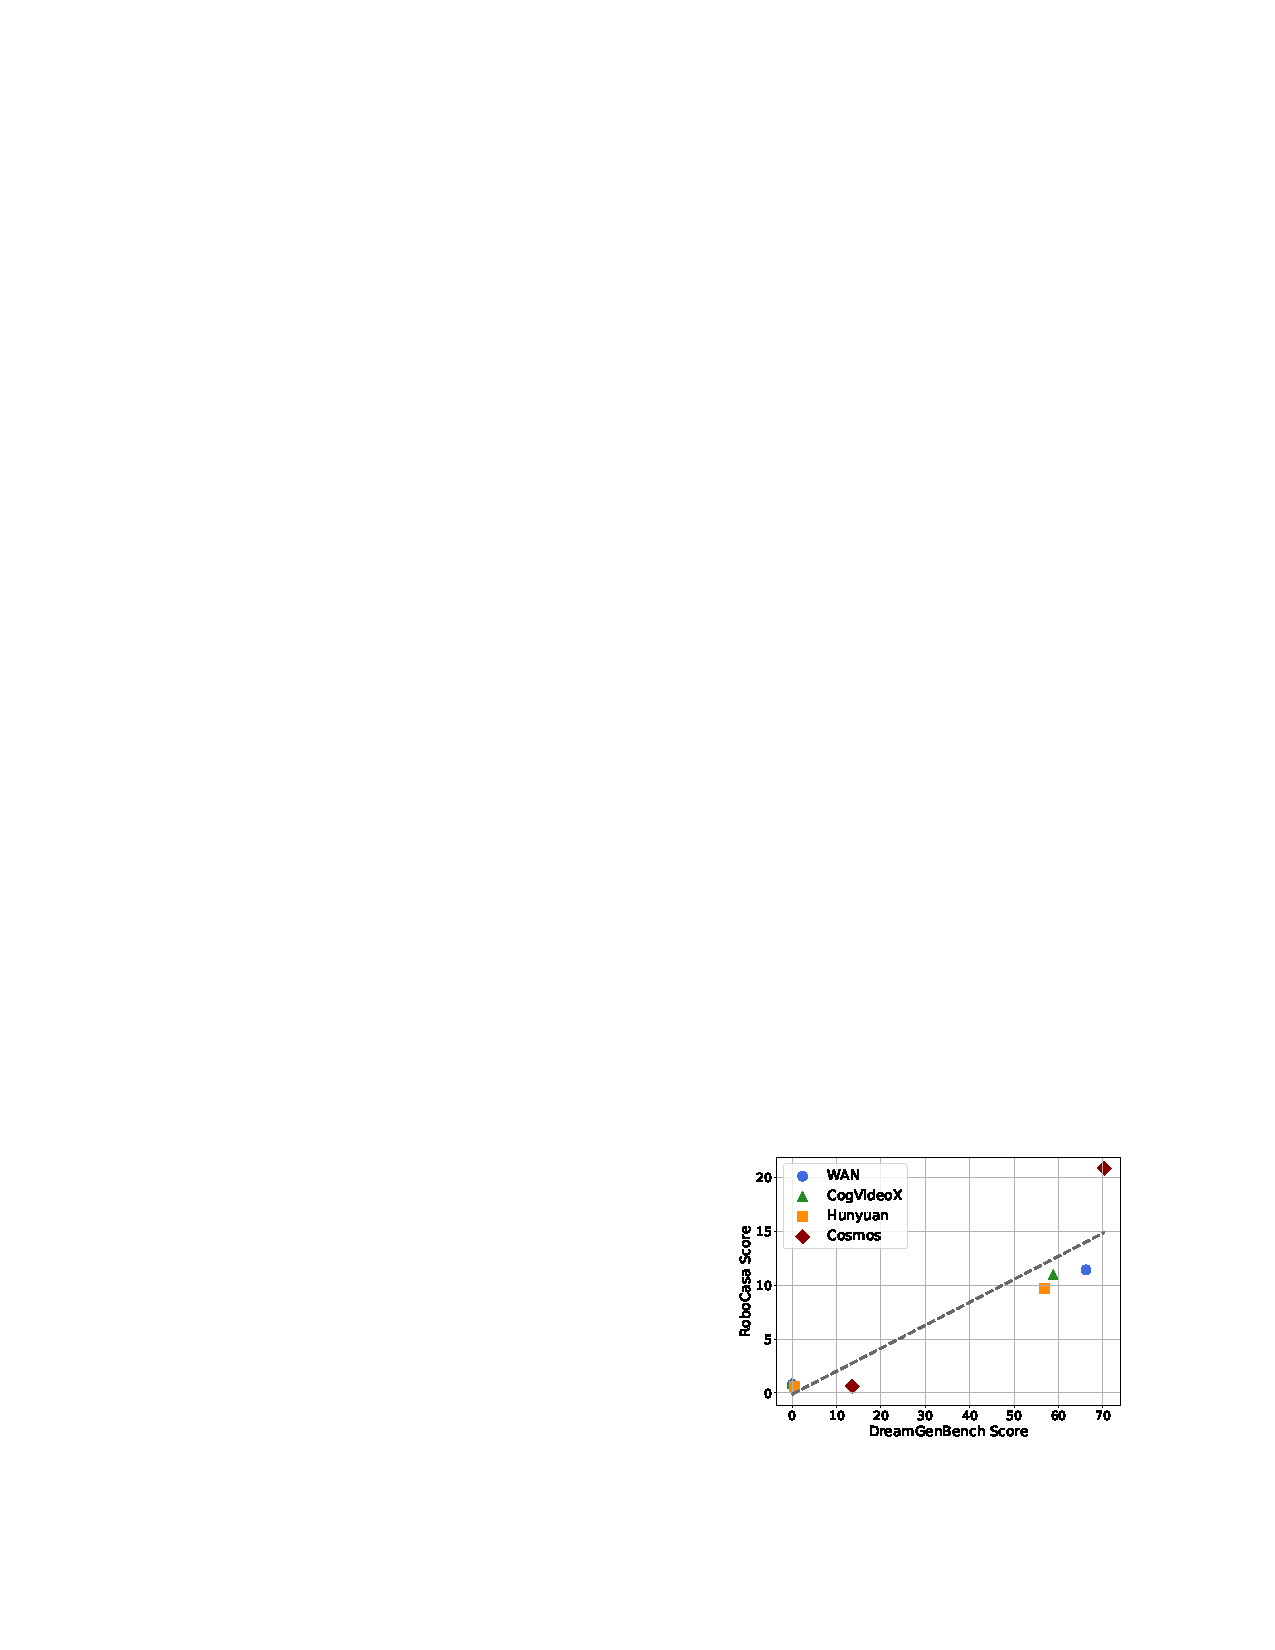
\includegraphics[width=0.7\textwidth,keepaspectratio]{extracted/figure_06.pdf}

      \captionof{figure}{Figure 6 (p.8) shows a positive correlation between DreamGen Bench scores and RoboCasa policy performance across different video world models.}
    \end{column}
  \end{columns}
\end{frame}

%------------------------------------------------
% TABLE 3
\begin{frame}
  \frametitle{LAPA Training Dataset Mix (Table 3)}
  \begin{columns}
    \begin{column}{0.45\textwidth}
      \small
      \begin{itemize}
        \item Table 3 (p.15) lists datasets used to train LAPA latent action model:
          \begin{itemize}
            \item Real robot: GR-1 Teleop, DROID, RT-1, Language Table, Bridge-v2, Agibot-Alpha
            \item Simulation: DexMG, RoboCasa
            \item Human: Something-Something v2, Ego4D
          \end{itemize}
        \item Total: 438.1M frames, 5{,}721.3 hours of video
        \item Diverse sources help latent actions capture general visual deltas across robots and humans
        \item LAPA uses codebook size 8, sequence length 16, trained 100k steps with batch size 1024
      \end{itemize}
    \end{column}
    \begin{column}{0.55\textwidth}
      \centering

      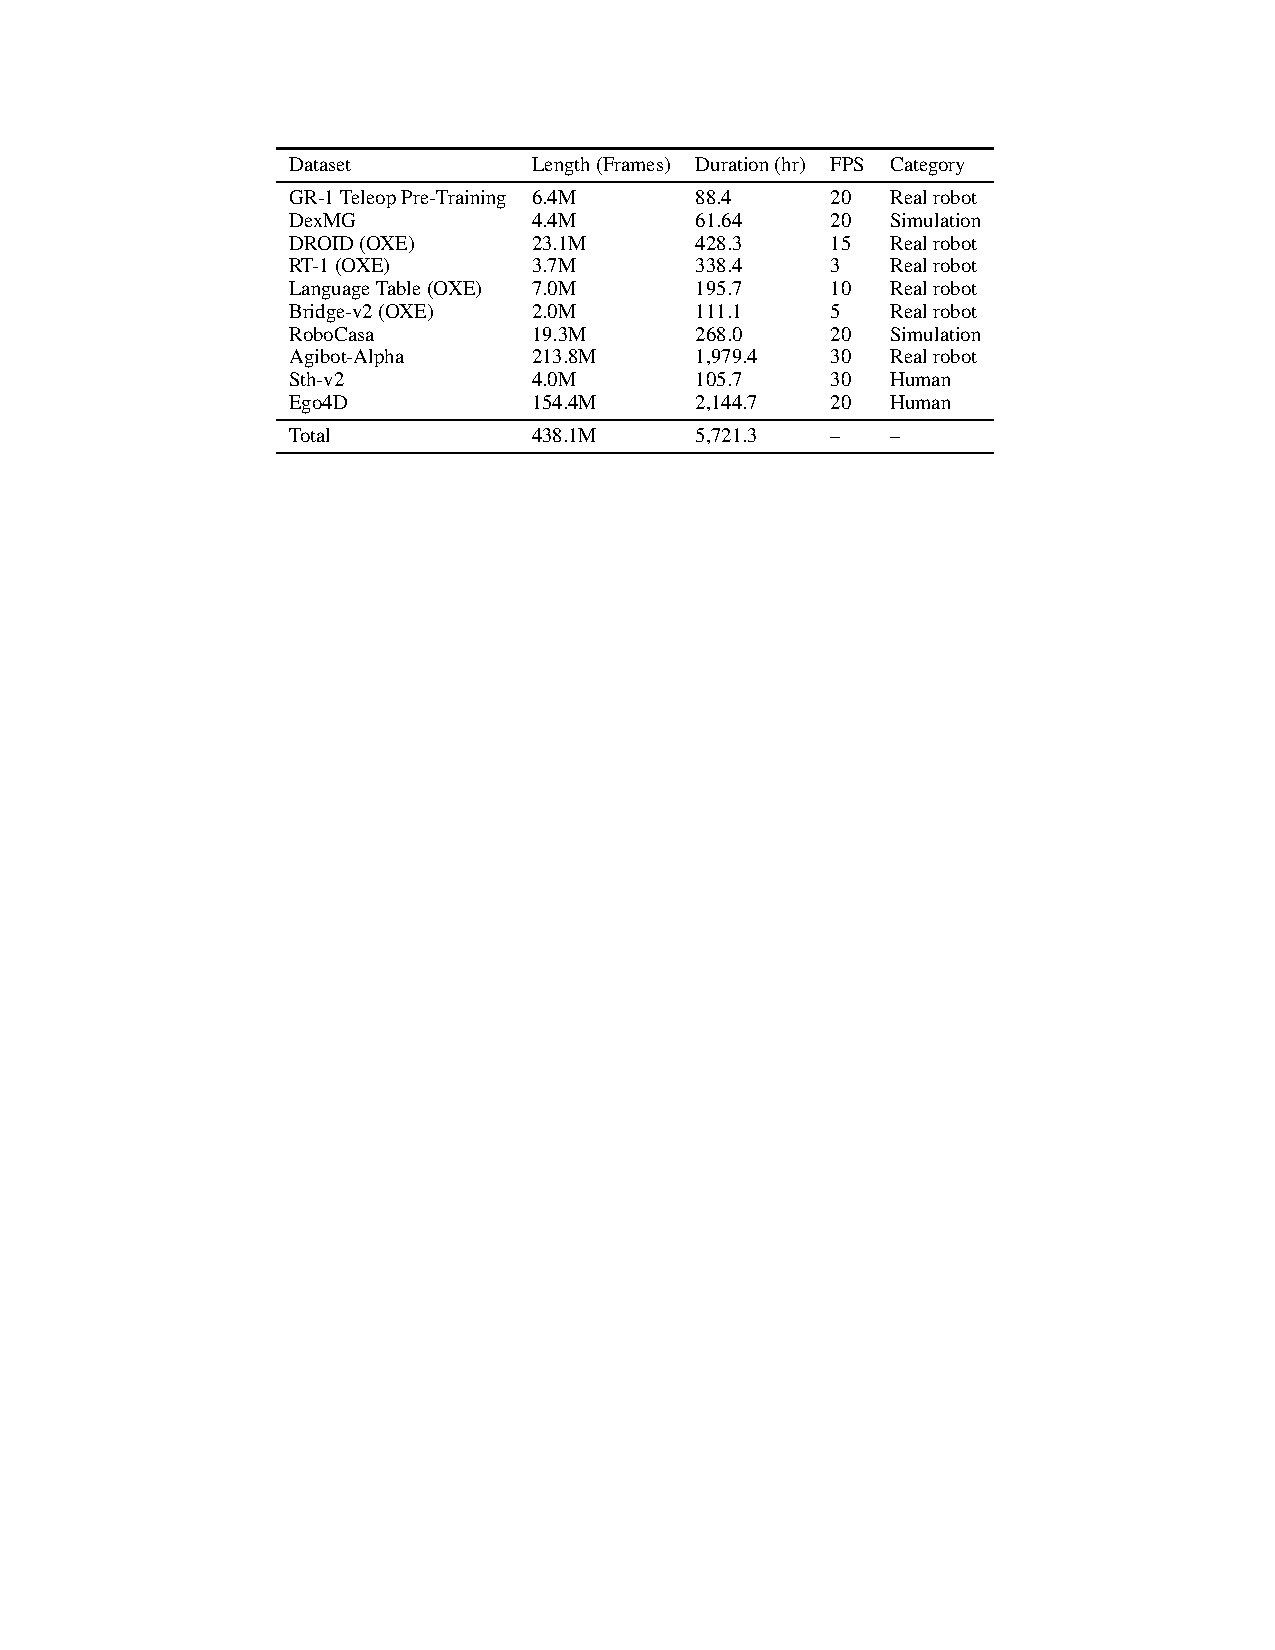
\includegraphics[width=0.9\columnwidth,keepaspectratio]{extracted/table_03.pdf}

      \captionof{figure}{Table 3 (p.15) provides statistics of datasets used to train the LAPA latent action model, including frame counts, durations, and categories.}
    \end{column}
  \end{columns}
\end{frame}

%------------------------------------------------
% FIGURE 7
\begin{frame}
  \frametitle{Neural Trajectories vs.\ Replay (Figure 7)}
  \begin{columns}
    \begin{column}{0.5\textwidth}
      \small
      \begin{itemize}
        \item Figure 7 (p.15) compares:
          \begin{itemize}
            \item Neural trajectories generated by WAN and CogVideoX
            \item Corresponding IDM action replays in simulation
          \end{itemize}
        \item Instruction: ``Use the right hand to pick up the plastic pitcher and pour water onto the green plant.''
        \item Replays allow diagnosing whether failures stem from:
          \begin{itemize}
            \item Video world model (poor language/physics)
            \item IDM quality
          \end{itemize}
        \item Authors observe most bottlenecks come from neural trajectory quality, highlighting importance of better video models
      \end{itemize}
    \end{column}
    \begin{column}{0.5\textwidth}
      \centering

      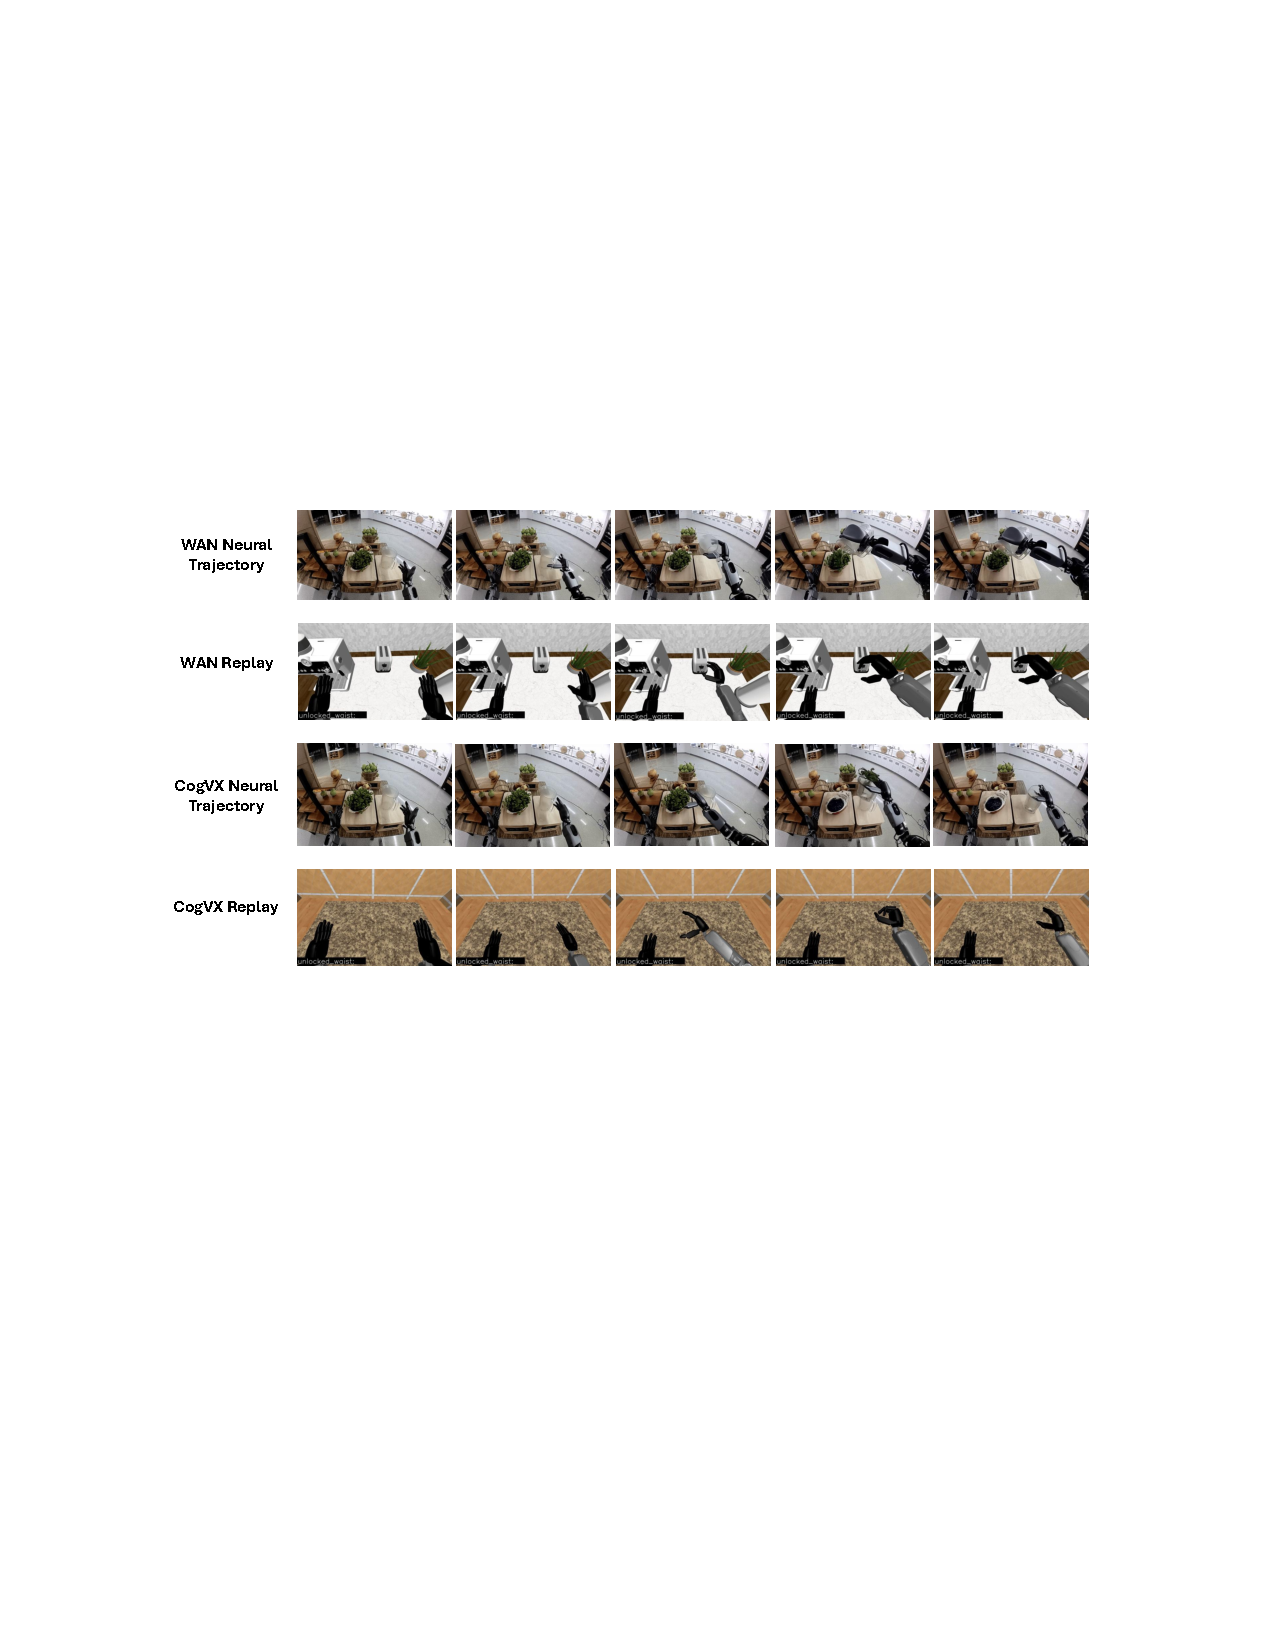
\includegraphics[width=0.7\textwidth,keepaspectratio]{extracted/figure_07.pdf}

      \captionof{figure}{Figure 7 (p.15) shows example neural trajectories and corresponding IDM action replays for WAN and CogVideoX on a pouring task.}
    \end{column}
  \end{columns}
\end{frame}

%------------------------------------------------
% FIGURE 8
\begin{frame}
  \frametitle{Seen Environment for GR1 (Figure 8)}
  \begin{columns}
    \begin{column}{0.5\textwidth}
      \small
      \begin{itemize}
        \item Figure 8 (p.16) shows sample images of the environment used to collect GR1 pick-and-place teleoperation data
        \item Single lab setup with tabletop, objects, and humanoid robot
        \item This environment is the only one used for training the video world model for GR1
        \item Environment generalization experiments use initial frames from other, unseen environments (Fig. 9)
      \end{itemize}
    \end{column}
    \begin{column}{0.5\textwidth}
      \centering

      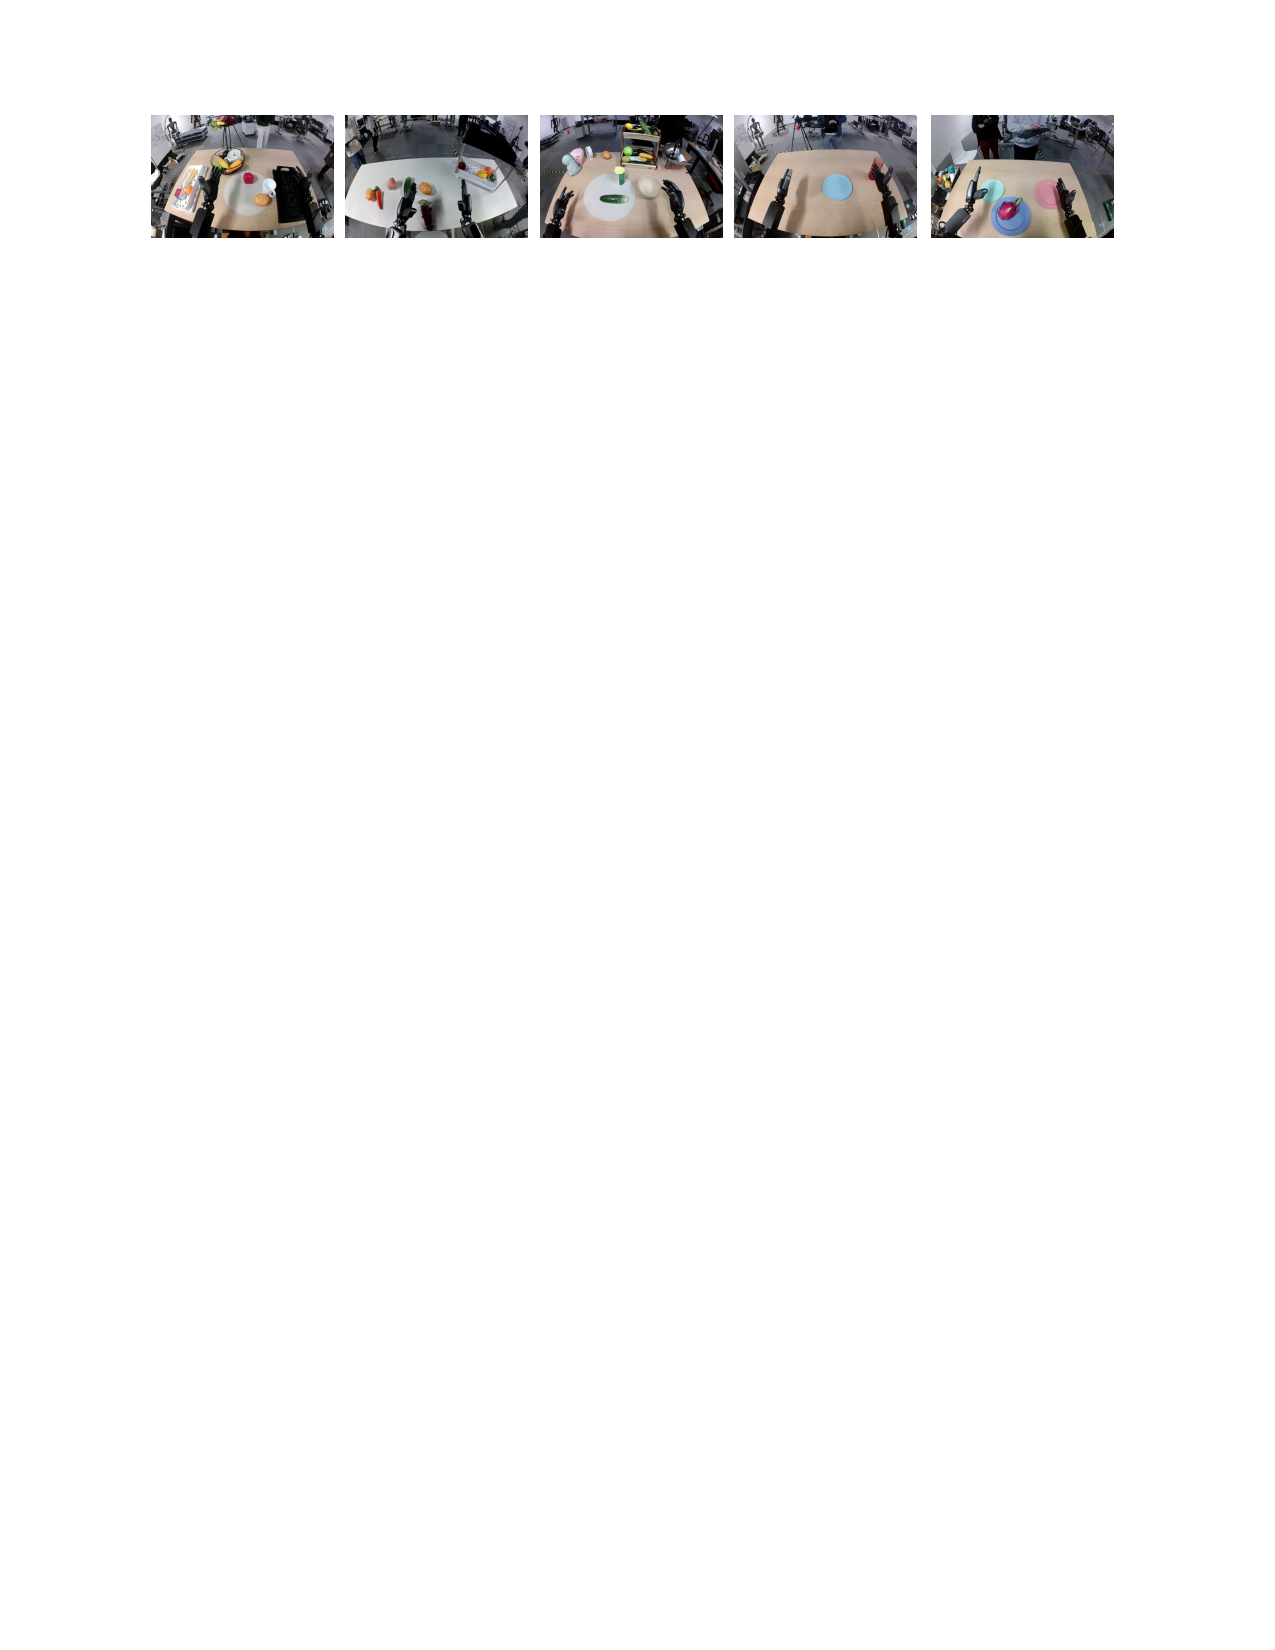
\includegraphics[width=0.7\textwidth,keepaspectratio]{extracted/figure_08.pdf}

      \captionof{figure}{Figure 8 (p.16) shows the seen environment where GR1 pick-and-place teleoperation data were collected.}
    \end{column}
  \end{columns}
\end{frame}

%------------------------------------------------
% FIGURE 9
\begin{frame}
  \frametitle{Unseen Environments for GR1 (Figure 9)}
  \begin{columns}
    \begin{column}{0.5\textwidth}
      \small
      \begin{itemize}
        \item Figure 9 (p.16) displays all 10 unseen environments used for environment generalization experiments
        \item Diverse layouts, backgrounds, and object configurations
        \item Video world model is \emph{not} trained on these environments; only initial frames are captured
        \item Policies trained solely on neural trajectories generated from these initial frames achieve non-trivial success (Table 1)
      \end{itemize}
    \end{column}
    \begin{column}{0.5\textwidth}
      \centering

      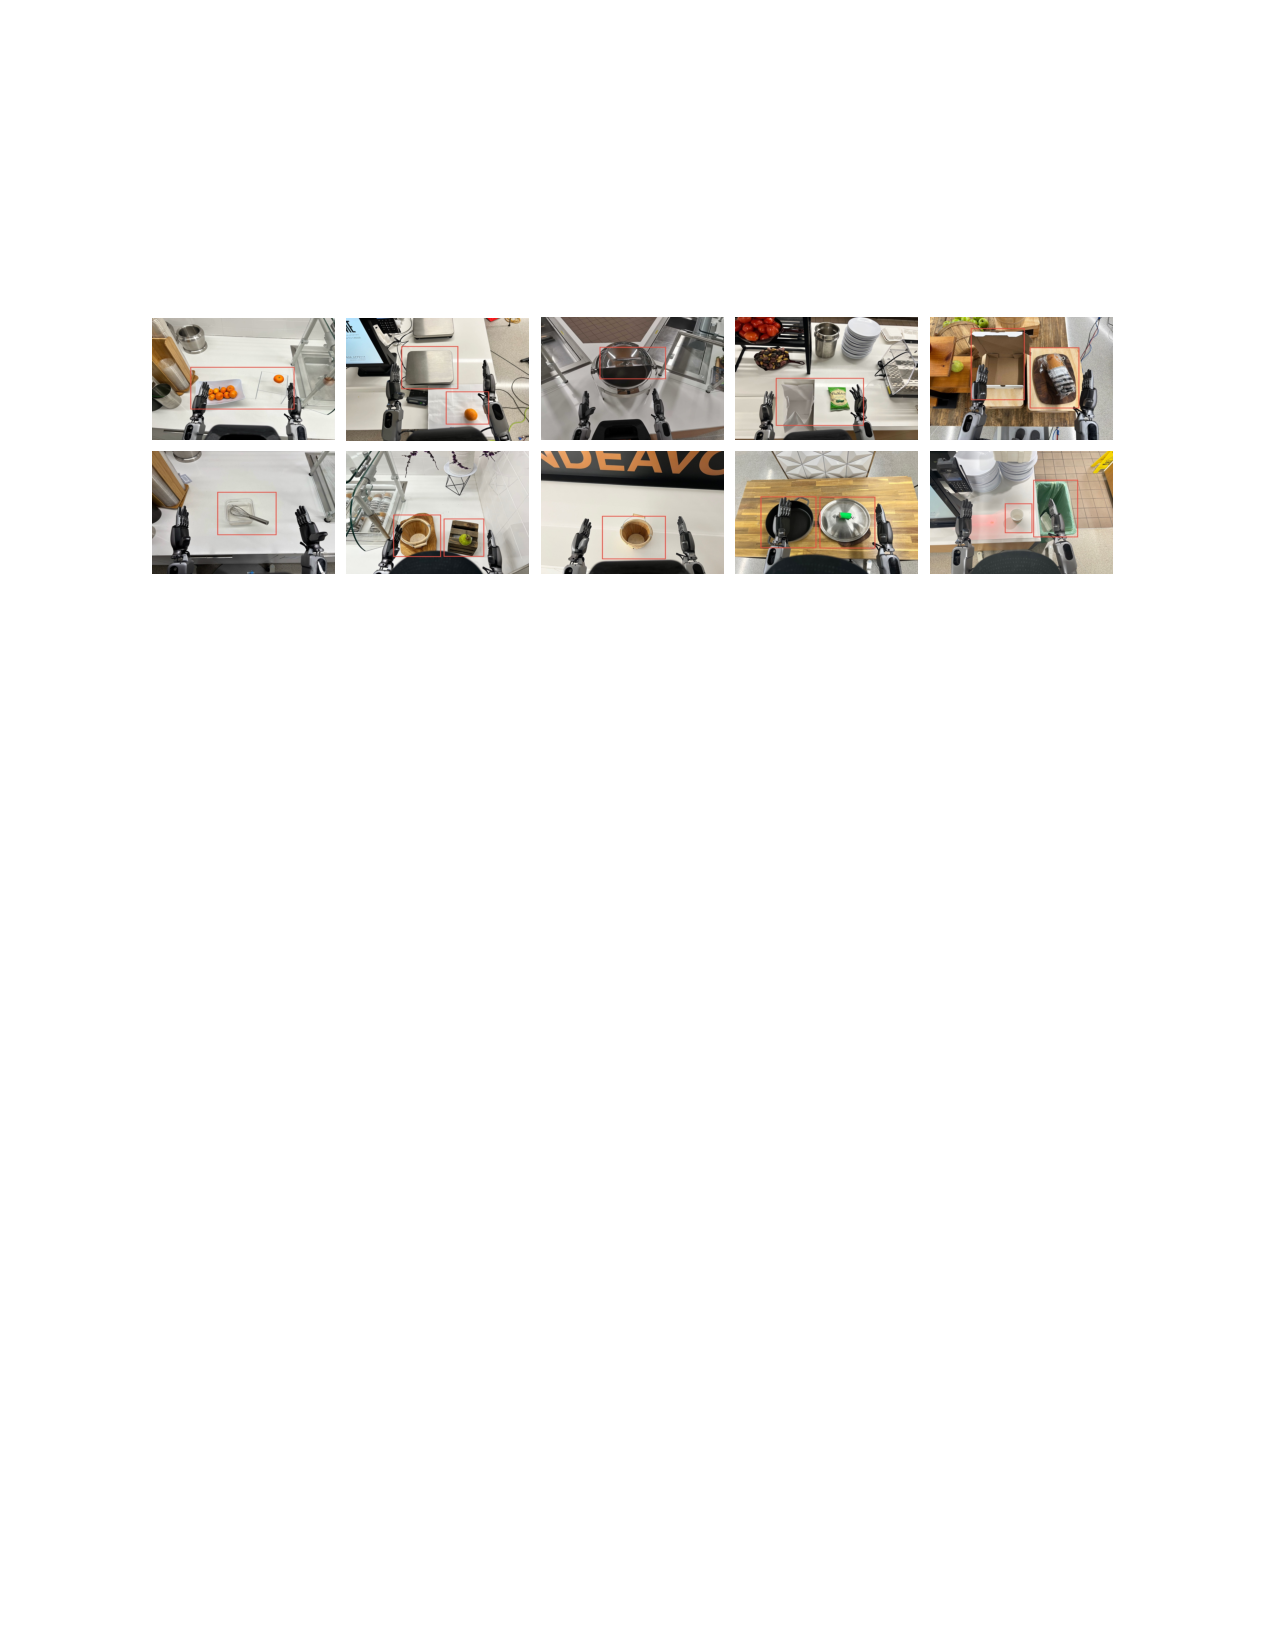
\includegraphics[width=0.7\textwidth,keepaspectratio]{extracted/figure_09.pdf}

      \captionof{figure}{Figure 9 (p.16) shows the 10 unseen environments used to evaluate environment generalization of GR1 policies.}
    \end{column}
  \end{columns}
\end{frame}

%------------------------------------------------
% FIGURE 10
\begin{frame}
  \frametitle{Multiview Data Processing (Figure 10)}
  \begin{columns}
    \begin{column}{0.5\textwidth}
      \small
      \begin{itemize}
        \item Figure 10 (p.16) illustrates multiview trajectories from:
          \begin{itemize}
            \item RoboCasa (top row)
            \item DROID (bottom row)
          \end{itemize}
        \item Views are arranged into a 2$\times$2 grid:
          \begin{itemize}
            \item Top-left: left camera
            \item Top-right: right camera
            \item Bottom-left: wrist camera
            \item Bottom-right: black image
          \end{itemize}
        \item This grid is used as input to video world models during fine-tuning and generation
      \end{itemize}
    \end{column}
    \begin{column}{0.5\textwidth}
      \centering

      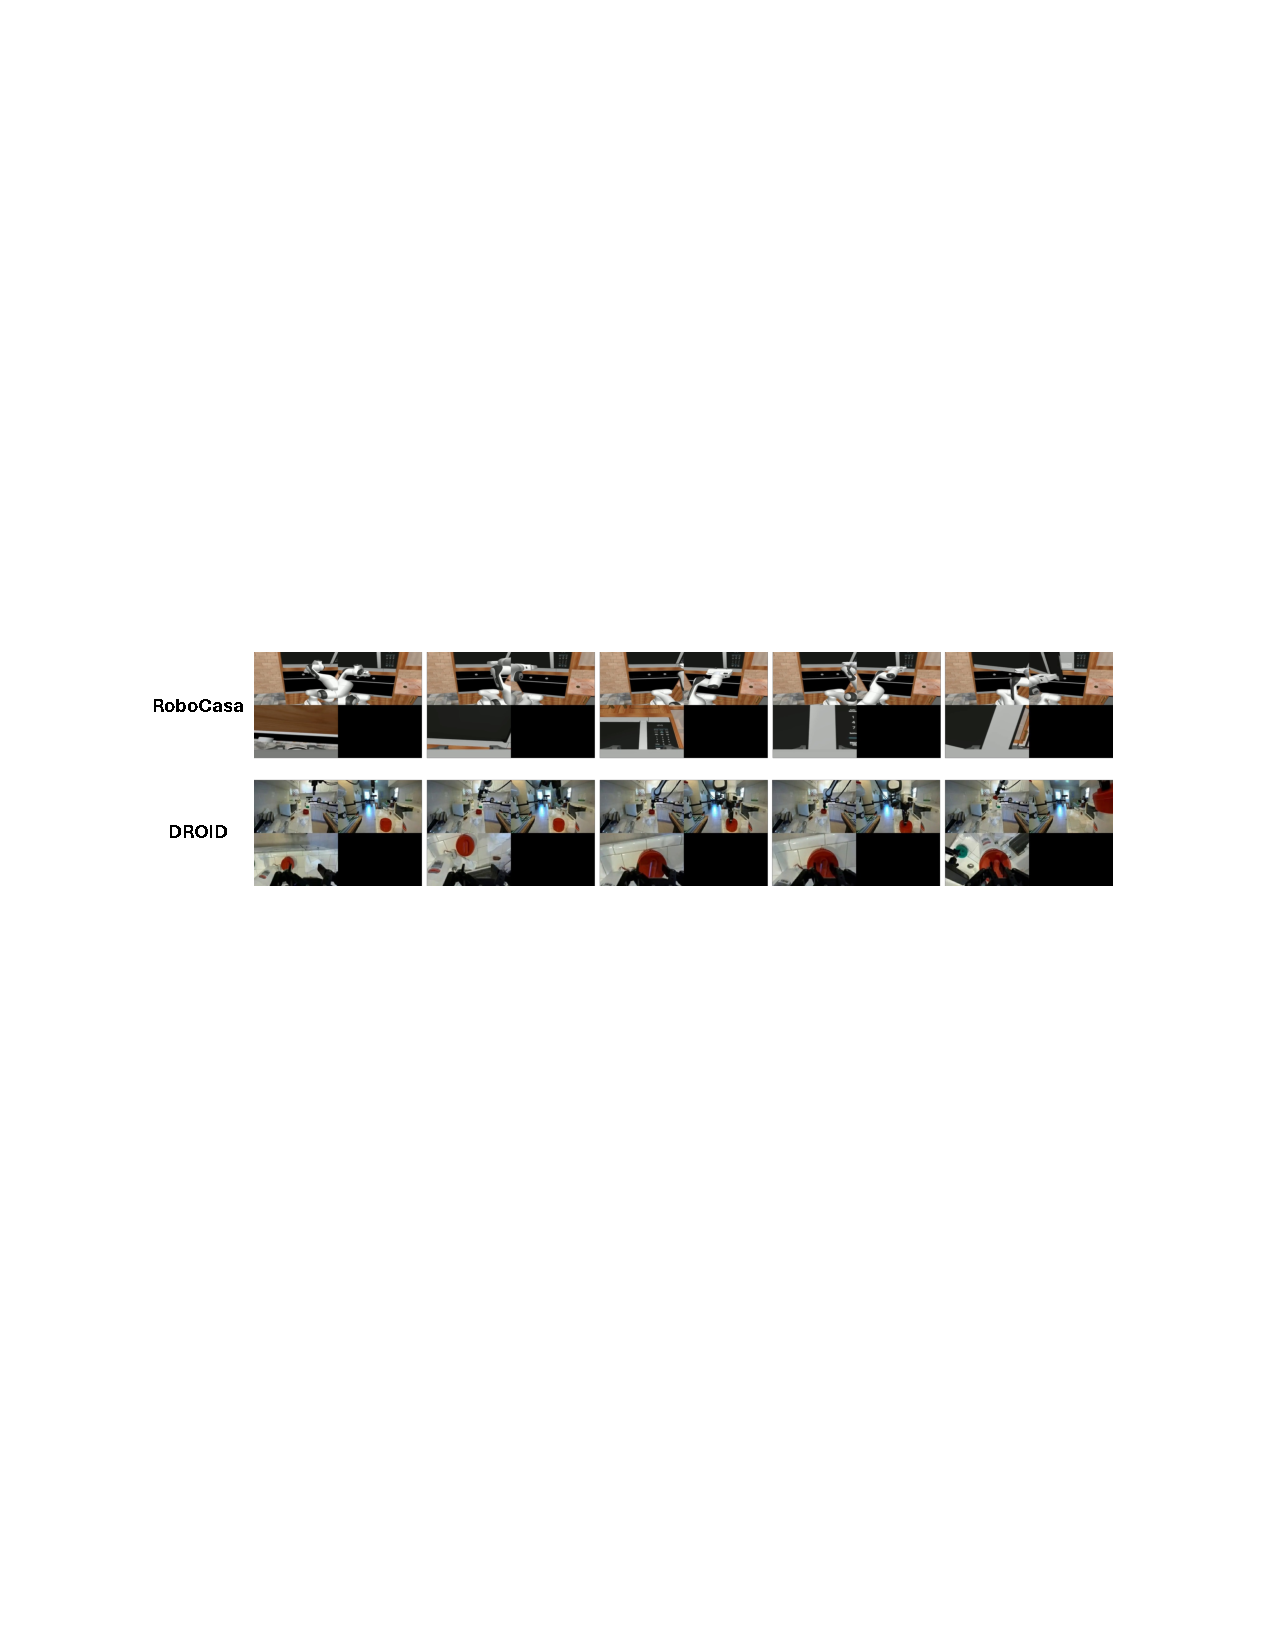
\includegraphics[width=0.7\textwidth,keepaspectratio]{extracted/figure_10.pdf}

      \captionof{figure}{Figure 10 (p.16) shows examples of multiview robot data from RoboCasa and DROID arranged into 2$\times$2 grids.}
    \end{column}
  \end{columns}
\end{frame}

%------------------------------------------------
% TABLE 4
\begin{frame}
  \frametitle{Detailed RoboCasa Results (Table 4)}
  \begin{columns}
    \begin{column}{0.45\textwidth}
      \small
      \begin{itemize}
        \item Table 4 (p.17) reports success rates for 24 RoboCasa tasks under:
          \begin{itemize}
            \item Different numbers of ground-truth trajectories (30, 100, 300)
            \item With and without 240k neural trajectories (NT)
            \item ``ONLY NT'': policies trained solely on neural trajectories
          \end{itemize}
        \item Co-training with NT consistently improves performance across tasks (e.g., door opening, drawer closing, knob turning)
        \item ONLY NT achieves 20.55\% average success, close to low-data baselines
        \item Some tasks (e.g., CloseDrawer, TurnOffMicrowave) reach high success ($>$80\%) with NT
      \end{itemize}
    \end{column}
    \begin{column}{0.55\textwidth}
      \centering

      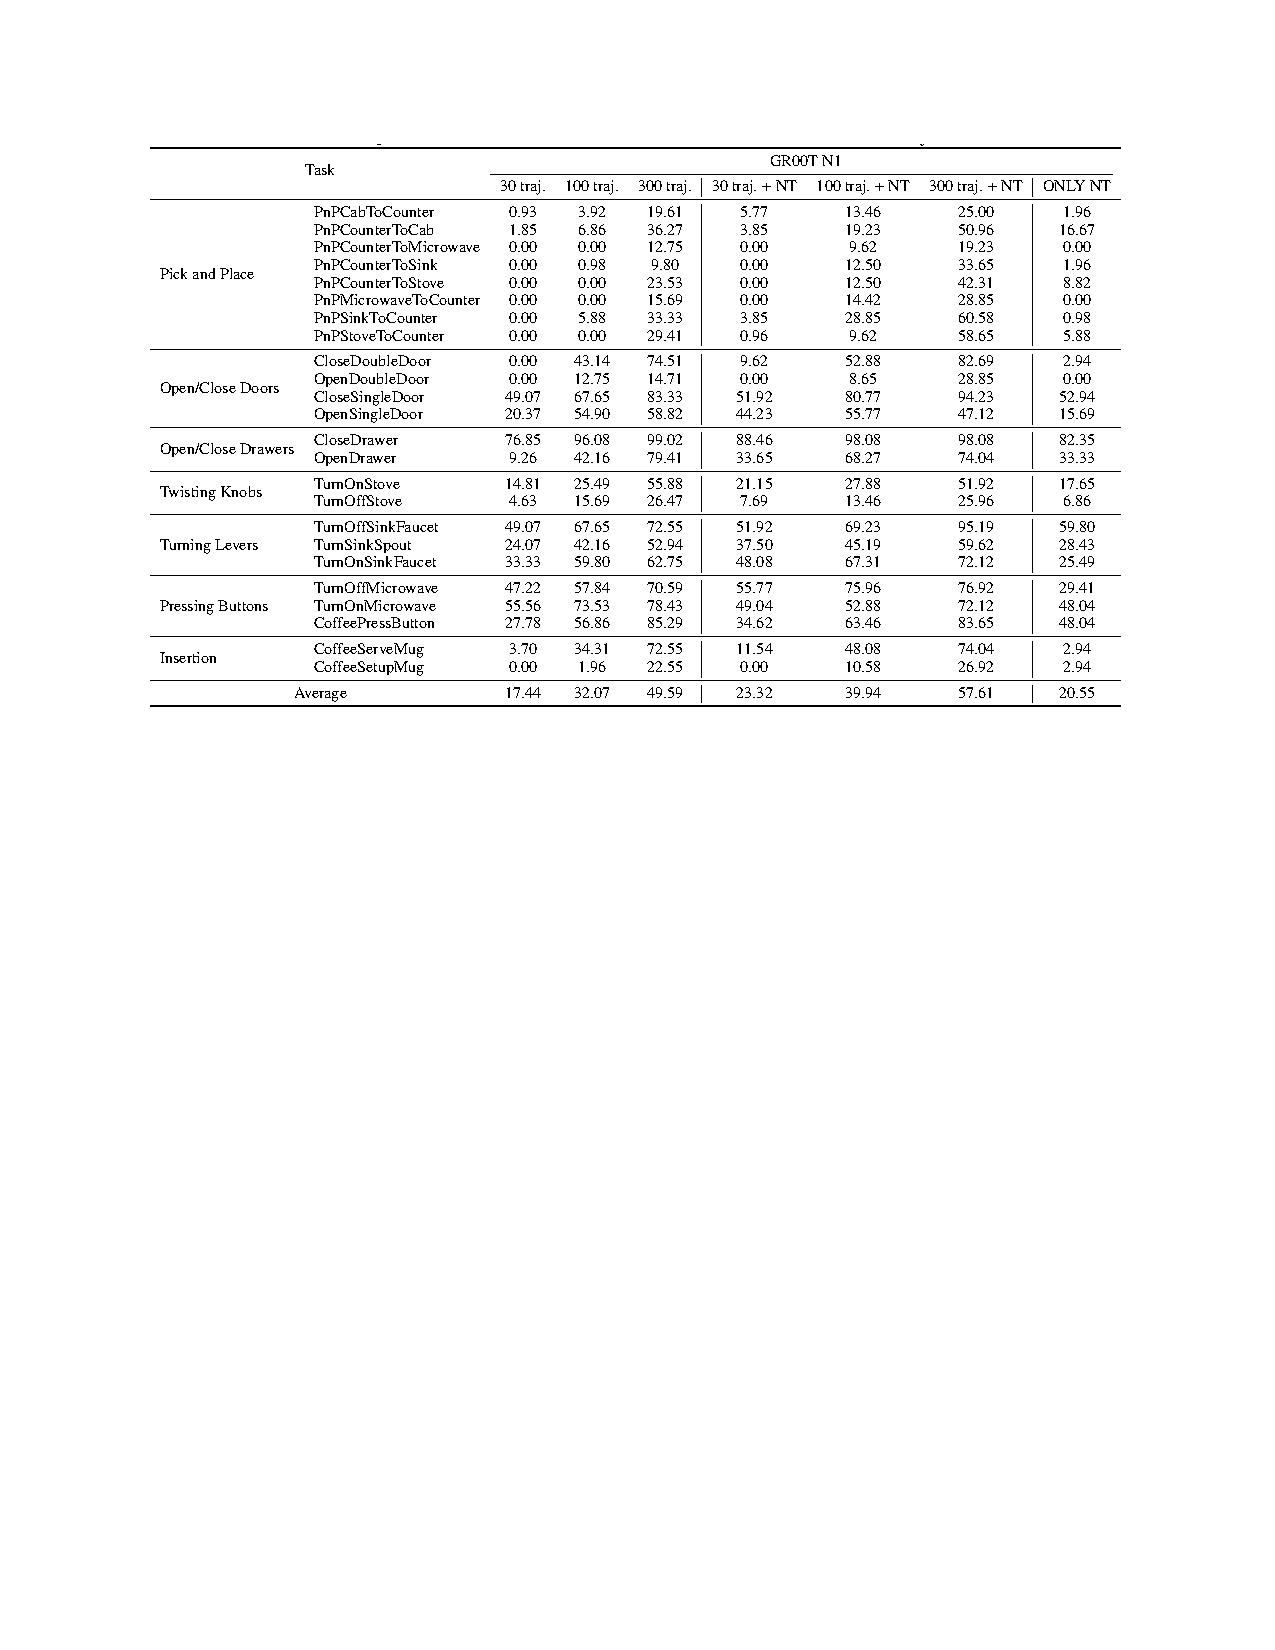
\includegraphics[width=0.9\columnwidth,keepaspectratio]{extracted/table_04.pdf}

      \captionof{figure}{Table 4 (p.17) lists per-task RoboCasa success rates for GR00T N1 under various ground-truth data sizes and with/without 240k neural trajectories.}
    \end{column}
  \end{columns}
\end{frame}

%------------------------------------------------
% TABLE 5
\begin{frame}
  \frametitle{Full Real-World Results (Table 5)}
  \begin{columns}
    \begin{column}{0.45\textwidth}
      \small
      \begin{itemize}
        \item Table 5 (p.18) shows success rates for:
          \begin{itemize}
            \item GR1 (Hammering, Wiping, Folding, Stacking)
            \item Franka (Pick\&Place, Cube Stacking, Tool Usage)
            \item SO-100 (Strawberry Pick\&Place, Tic-Tac-Toe)
          \end{itemize}
        \item Compares:
          \begin{itemize}
            \item DP, $\pi_0$, GR00T N1
            \item With and without neural trajectories
            \item High Data (100\% real trajectories) baselines
          \end{itemize}
        \item Neural trajectories improve low-data performance; e.g., GR00T N1 average on GR1: 37.0\% $\rightarrow$ 46.0\%
        \item High Data still yields best performance, but DREAMGEN narrows the gap with far fewer real trajectories
      \end{itemize}
    \end{column}
    \begin{column}{0.55\textwidth}
      \centering

      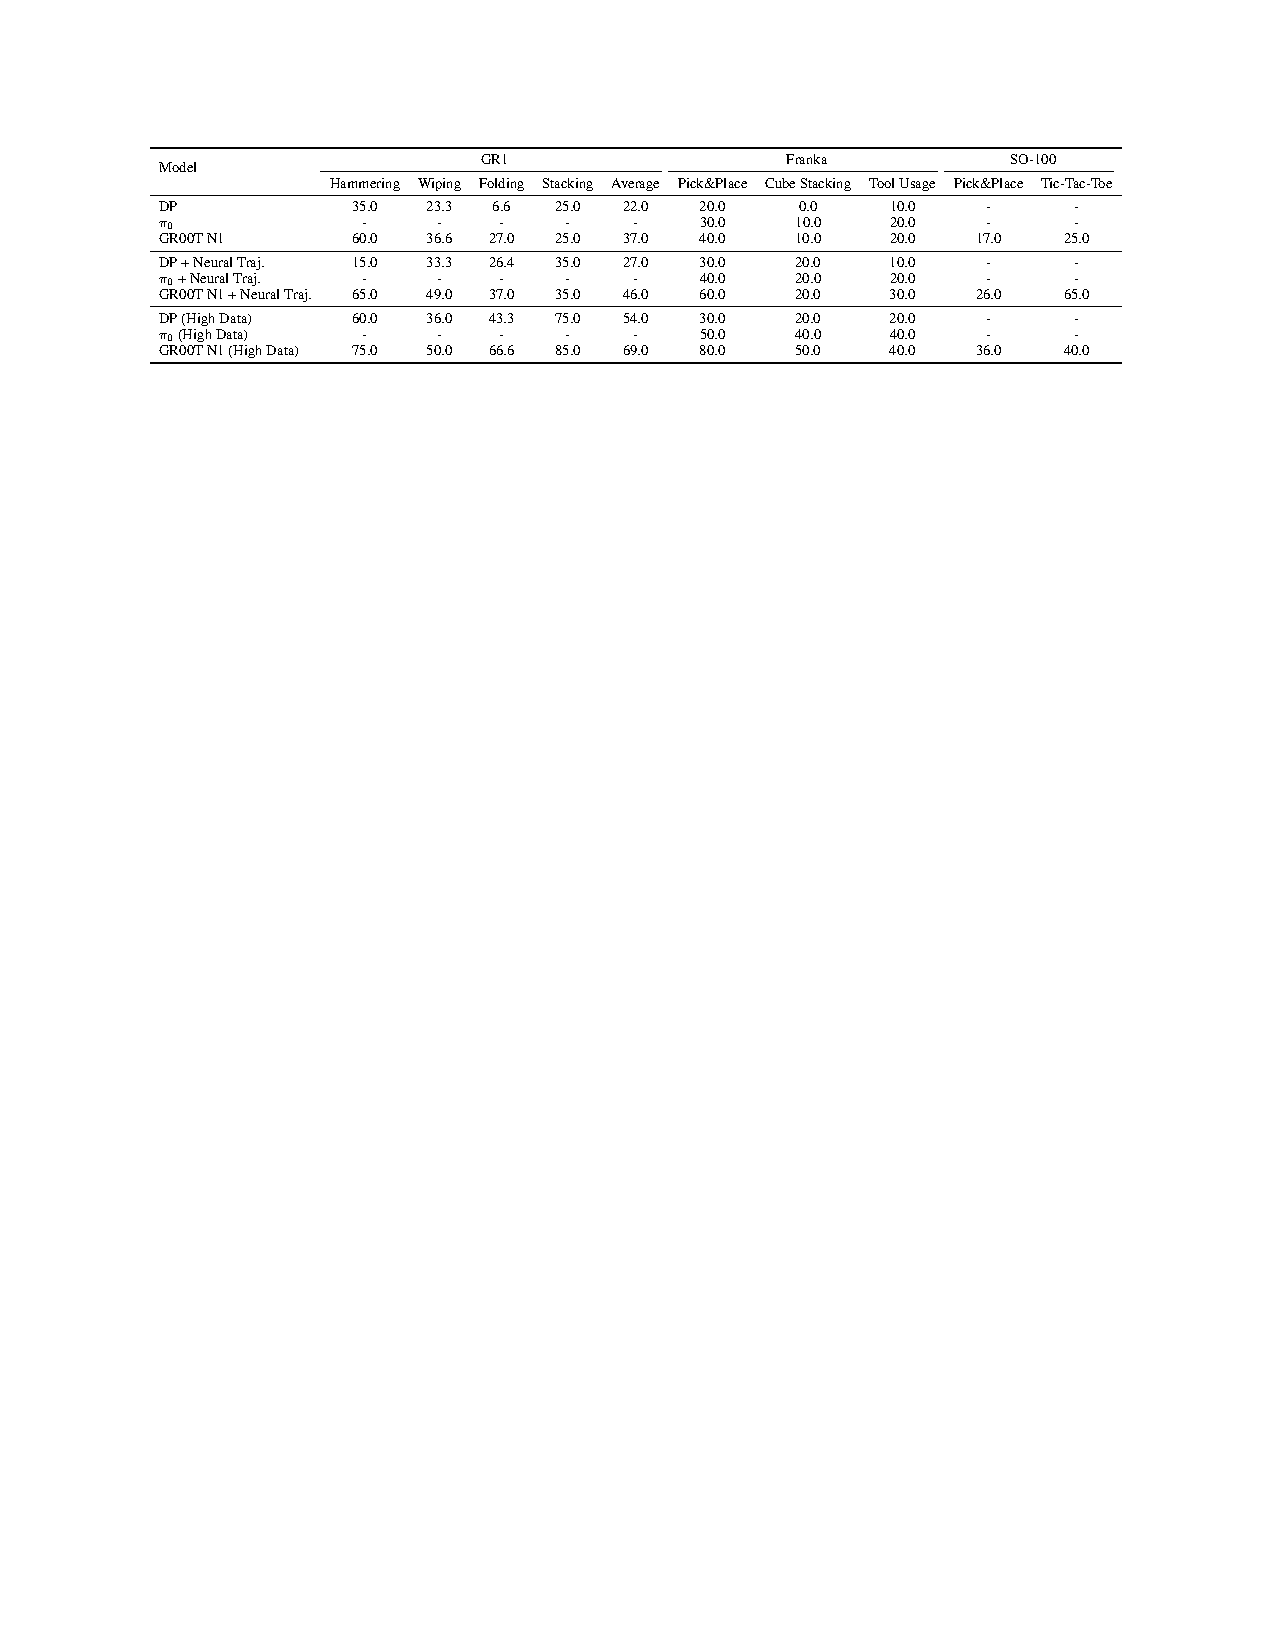
\includegraphics[width=0.9\columnwidth,keepaspectratio]{extracted/table_05.pdf}

      \captionof{figure}{Table 5 (p.18) reports success rates for real-world GR1, Franka, and SO-100 tasks across models, with/without neural trajectories, and with High Data.}
    \end{column}
  \end{columns}
\end{frame}

%------------------------------------------------
% FIGURE 11
\begin{frame}
  \frametitle{GR1 Evaluation Setups (Figure 11)}
  \begin{columns}
    \begin{column}{0.5\textwidth}
      \small
      \begin{itemize}
        \item Figure 11 (p.20) visualizes evaluation configurations for GR1:
          \begin{itemize}
            \item Seen environment, new behaviors (14 tasks)
            \item New environments, seen behaviors (6 tasks)
            \item New environments, new behaviors (7 tasks)
          \end{itemize}
        \item Rectangular boxes indicate regions where target objects are randomized during evaluation
        \item Same randomization protocol used across models for fair comparison
        \item Partial credit criteria for each task are detailed in Table 8 (p.21)
      \end{itemize}
    \end{column}
    \begin{column}{0.5\textwidth}
      \centering

      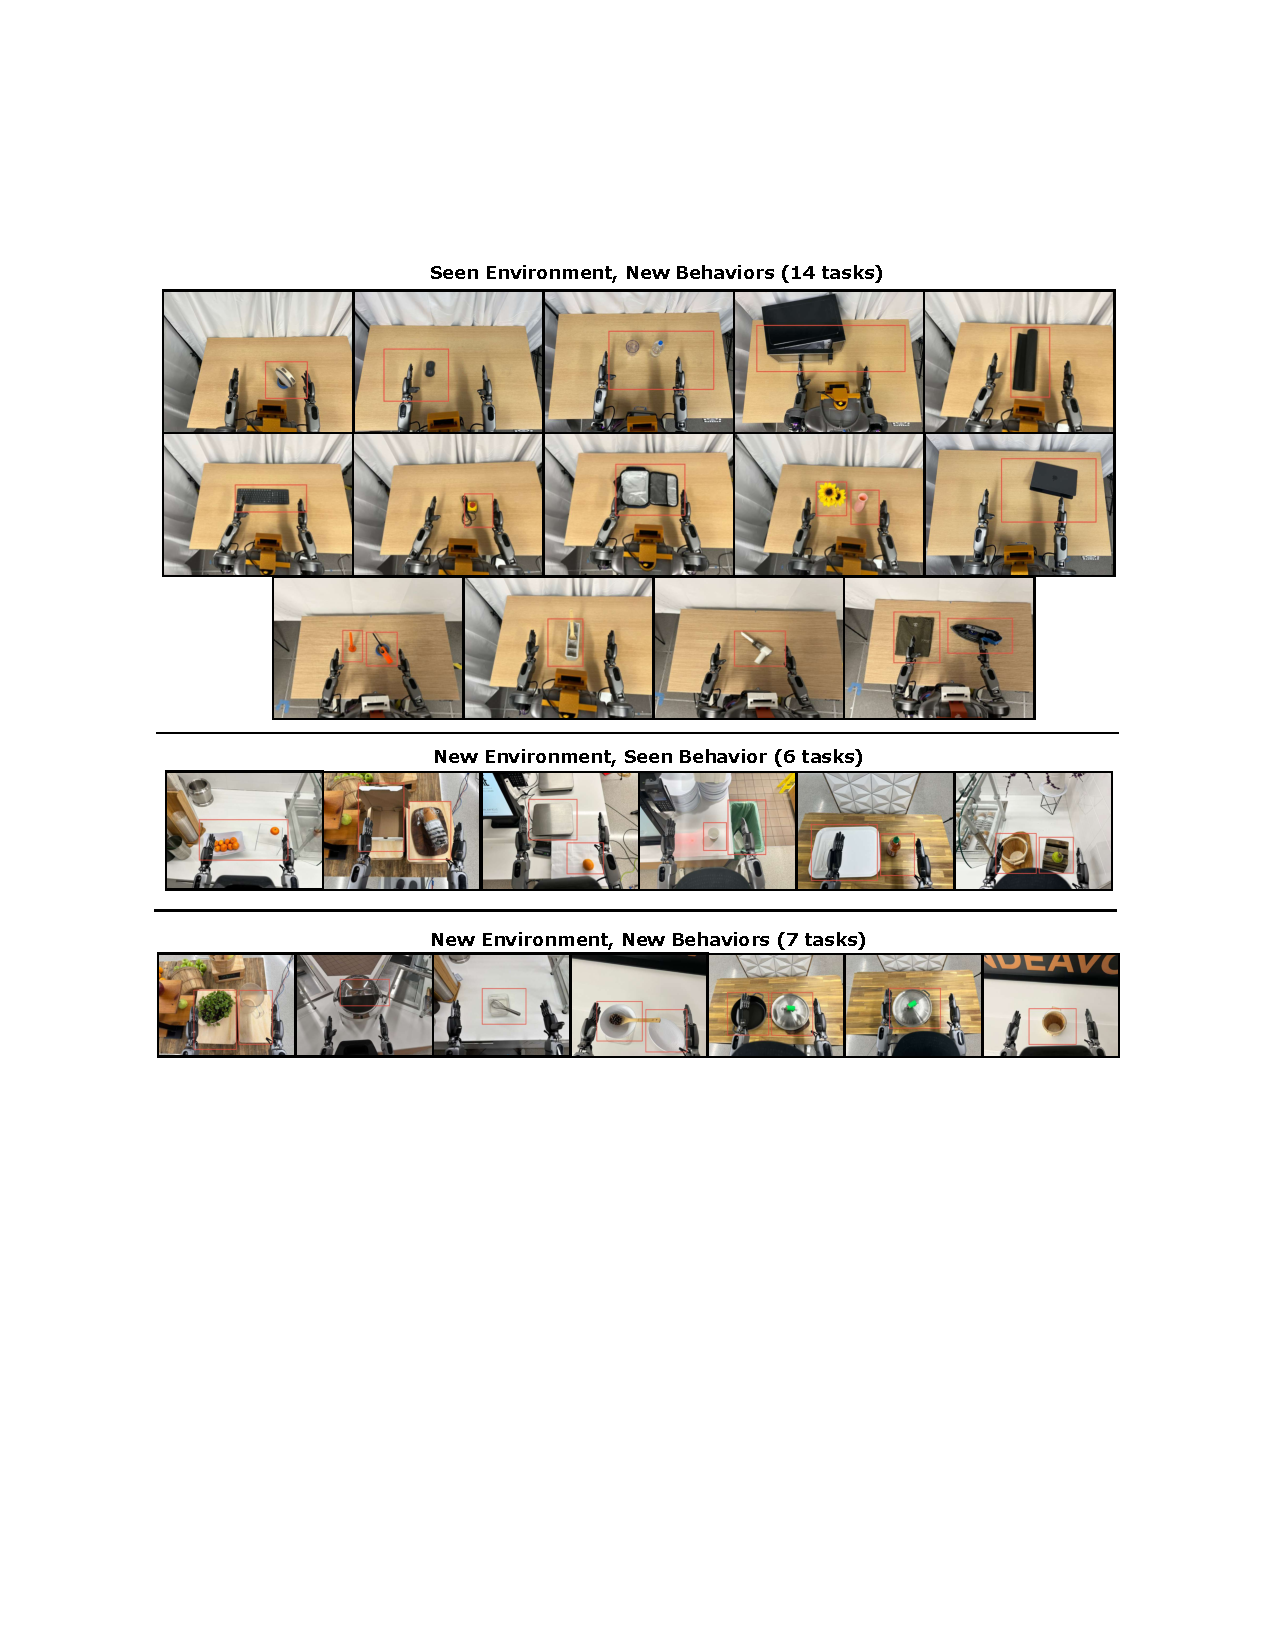
\includegraphics[width=0.7\textwidth,keepaspectratio]{extracted/figure_11.pdf}

      \captionof{figure}{Figure 11 (p.20) shows evaluation setups and object randomization regions for GR1 behavior and environment generalization experiments.}
    \end{column}
  \end{columns}
\end{frame}

%------------------------------------------------
% TABLE 8
\begin{frame}
  \frametitle{GR1 Task Evaluation Criteria (Table 8)}
  \begin{columns}
    \begin{column}{0.45\textwidth}
      \small
      \begin{itemize}
        \item Table 8 (p.21) defines success metrics for GR1 generalization tasks:
          \begin{itemize}
            \item Seen env, novel behaviors (e.g., Open Microwave, Pour Water, Move Mouse)
            \item Novel env, seen behaviors (e.g., Pick up Tangerine, Put Cup in Trash)
            \item Novel env, novel behaviors (e.g., Use Whisk, Cover Pot)
          \end{itemize}
        \item Many tasks use graded scores (0.33, 0.5, 0.66, 1.0) for partial completion
        \item Ensures nuanced evaluation of complex, multi-stage behaviors
        \item 10 rollouts per checkpoint with randomized object locations
      \end{itemize}
    \end{column}
    \begin{column}{0.55\textwidth}
      \centering

      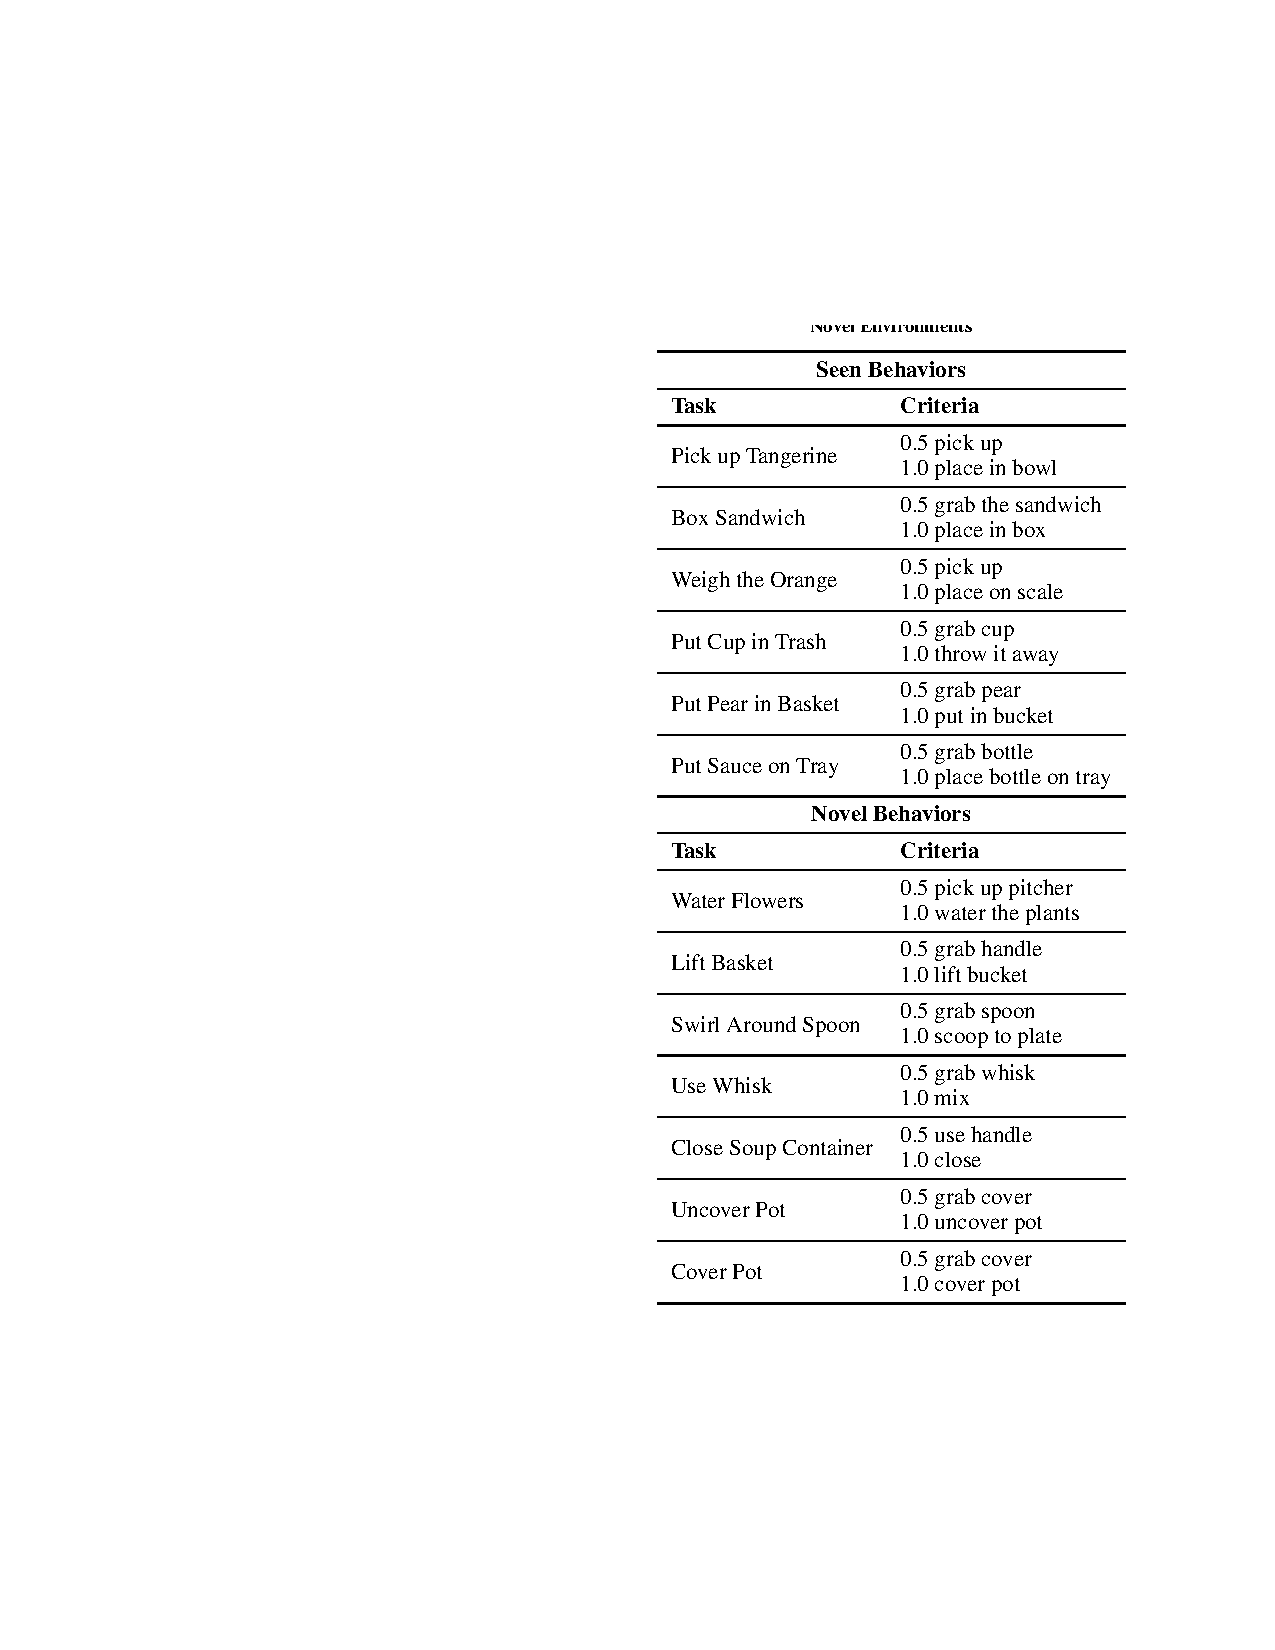
\includegraphics[width=0.9\columnwidth,keepaspectratio]{extracted/table_08.pdf}

      \captionof{figure}{Table 8 (p.21) specifies detailed evaluation criteria and partial credit schemes for GR1 behavior and environment generalization tasks.}
    \end{column}
  \end{columns}
\end{frame}

%------------------------------------------------
% FIGURE 12
\begin{frame}
  \frametitle{Examples of Neural Trajectories (Figure 12)}
  \begin{columns}
    \begin{column}{0.5\textwidth}
      \small
      \begin{itemize}
        \item Figure 12 (p.23) shows example neural trajectories for:
          \begin{itemize}
            \item Training data augmentation
            \item New behavior generalization
            \item New environment generalization
          \end{itemize}
        \item Sequences depict GR1 performing tasks such as:
          \begin{itemize}
            \item Pick-and-place variations
            \item Novel interactions with objects (e.g., tools, containers)
            \item Behaviors in visually distinct environments
          \end{itemize}
        \item Illustrates visual realism and diversity of generated trajectories used for policy training
      \end{itemize}
    \end{column}
    \begin{column}{0.5\textwidth}
      \centering

      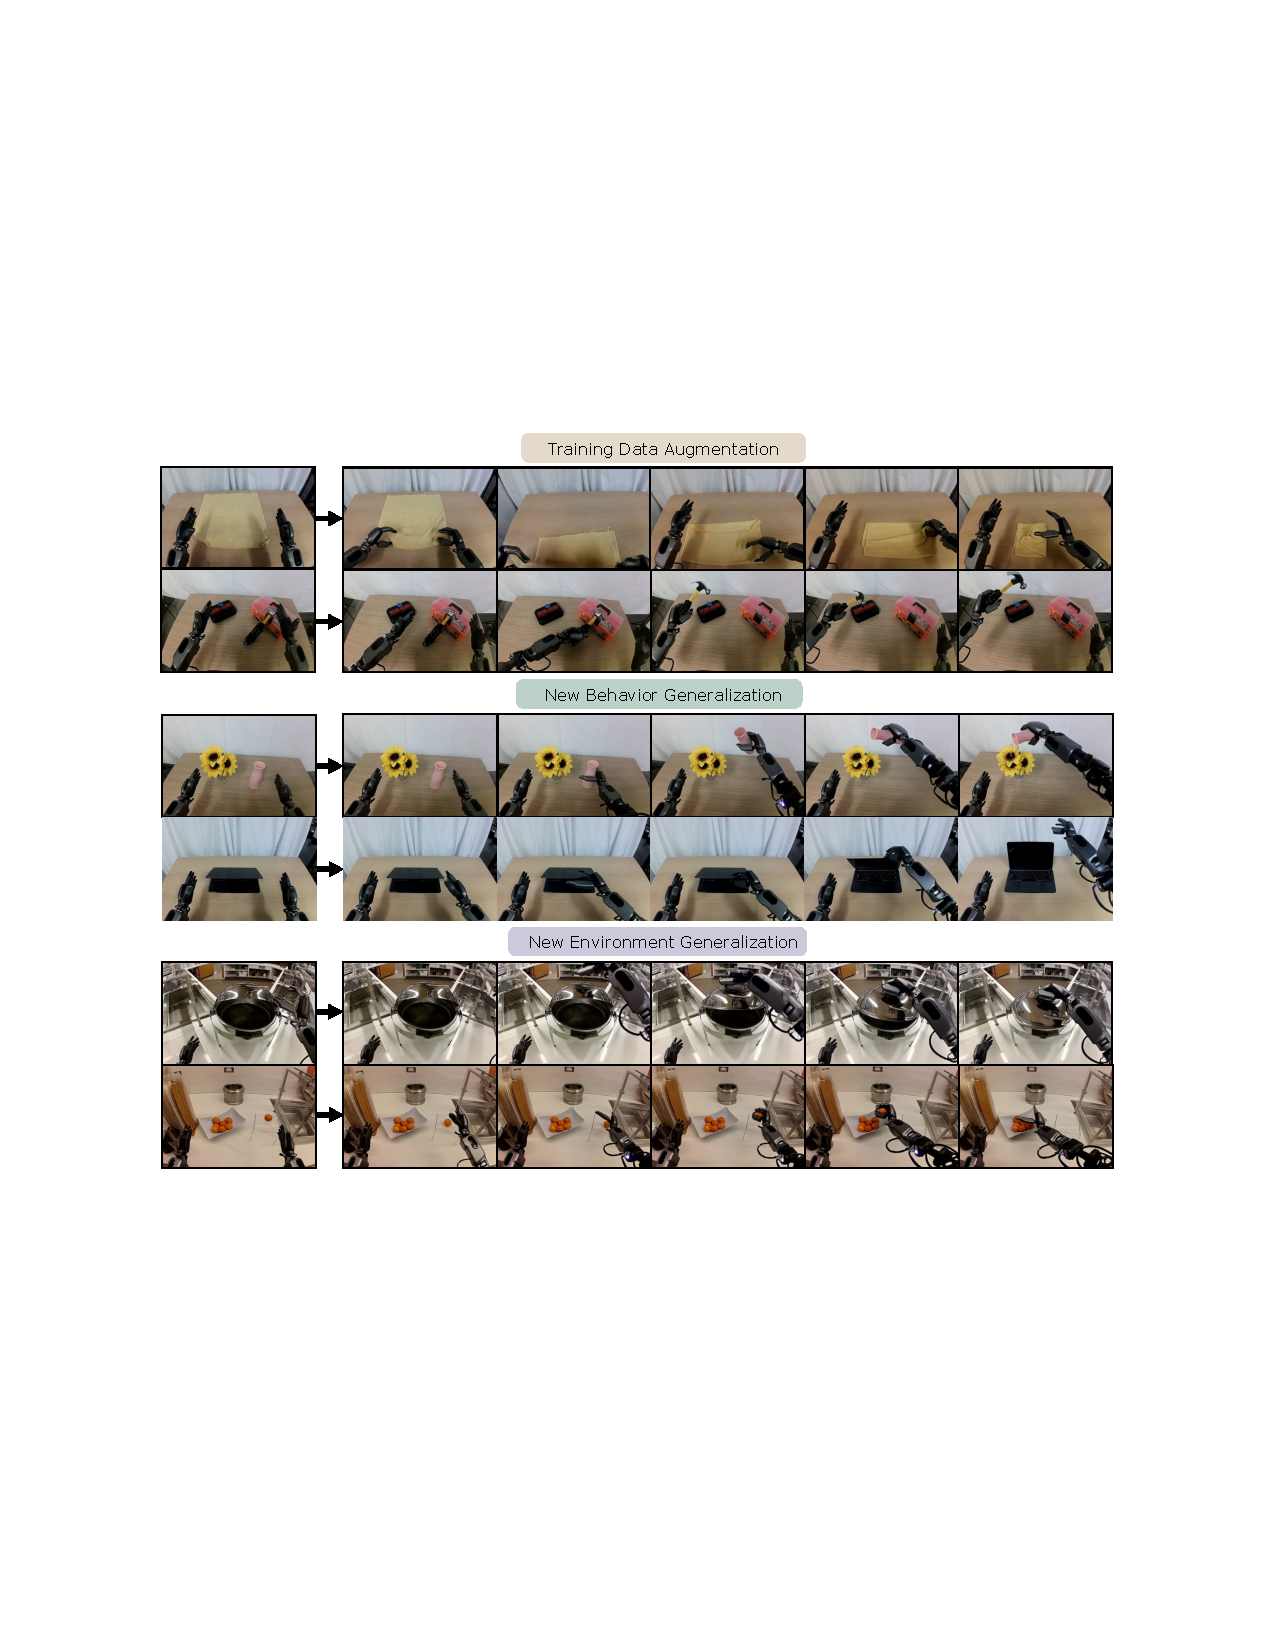
\includegraphics[width=0.7\textwidth,keepaspectratio]{extracted/figure_12.pdf}

      \captionof{figure}{Figure 12 (p.23) presents example neural trajectories for data augmentation, new behaviors, and new environments.}
    \end{column}
  \end{columns}
\end{frame}

%------------------------------------------------
\begin{frame}
  \frametitle{Key Results and Analysis}
  \small
  \begin{itemize}
    \item \textbf{Data augmentation}:
      \begin{itemize}
        \item RoboCasa: log-linear performance gains with more neural trajectories; ONLY NT reaches 20.55\% avg.\ success
        \item Real robots: consistent improvements across GR1, Franka, SO-100 with few real trajectories
      \end{itemize}
    \item \textbf{Behavior generalization}:
      \begin{itemize}
        \item GR1 learns 22 new behaviors from neural trajectories alone
        \item Success on novel verbs increases from 11.2\% to 43.2\% in seen environment
      \end{itemize}
    \item \textbf{Environment generalization}:
      \begin{itemize}
        \item From single training environment, policies achieve 28.5\% avg.\ success on tasks in 10 unseen environments
        \item Baseline GR00T N1 trained only on pick-and-place in one env achieves 0\% on these tasks
      \end{itemize}
    \item \textbf{DreamGen Bench}:
      \begin{itemize}
        \item IF/PA metrics correlate strongly with downstream policy performance
      \end{itemize}
  \end{itemize}
\end{frame}

%------------------------------------------------
\begin{frame}
  \frametitle{Conclusion}
  \small
  \begin{itemize}
    \item DREAMGEN uses video world models as scalable synthetic data generators for robot learning
    \item Neural trajectories (videos + pseudo-actions) enable:
      \begin{itemize}
        \item Effective data augmentation in simulation and real world
        \item Learning entirely new behaviors without additional teleoperation
        \item Zero-shot environment generalization from a single training environment
      \end{itemize}
    \item DreamGen Bench provides a practical benchmark linking video model quality to robot policy performance
    \item The work highlights a promising axis for scaling robot learning beyond manual data collection
  \end{itemize}
\end{frame}

%------------------------------------------------
\begin{frame}
  \frametitle{Limitations and Future Work}
  \small
  \begin{itemize}
    \item Current tasks are relatively simple and cover limited kinematic capabilities
    \item Supporting more complex, dexterous behaviors requires:
      \begin{itemize}
        \item Richer control
        \item More diverse training behaviors and video-language pairings
      \end{itemize}
    \item DREAMGEN is compute-intensive (e.g., 240k RoboCasa trajectories took 54 hours on 1500 NVIDIA L40 GPUs)
    \item Manual selection of initial frames introduces operational overhead
    \item Automatic evaluators in DreamGen Bench can hallucinate, especially for physical realism; improving evaluation remains open
    \item Zero-shot generalization to novel robots with no ground-truth data is still an open question
  \end{itemize}
\end{frame}

%------------------------------------------------
\begin{frame}
  \centering
  \Large Thank you!\\[1em]
  \normalsize Questions?
\end{frame}

%------------------------------------------------
\end{document}